\PassOptionsToPackage{unicode}{hyperref}
\documentclass[aspectratio=1610, 9pt]{beamer}

% Load packages you need here
\usepackage{polyglossia}
\setmainlanguage{english}

\usepackage{csquotes}
    

\usepackage{amsmath}
\usepackage{amssymb}
\usepackage{mathtools}

\usepackage{hyperref}
\usepackage{bookmark}
\usepackage[
  locale=UK,
  separate-uncertainty=true,
  per-mode=symbol-or-fraction,
]{siunitx}
\usepackage[
  backend=biber,   % use modern biber backend
  autolang=hyphen, % load hyphenation rules for if language of bibentry is not
  % german, has to be loaded with \setotherlanguages
  % in the references.bib use langid={en} for english sources
  sorting=none,
  ]{biblatex}
  \addbibresource{references.bib}  % the bib file to use
  \DefineBibliographyStrings{english}{andothers = {{et\,al\adddot}}}  % replace u.a. with et al.
  
  
% load the theme after all packages
\usetheme[
  showtotalframes, % show total number of frames in the footline
]{tudo}

% Put settings here, like
\unimathsetup{
  math-style=ISO,
  bold-style=ISO,
  nabla=upright,
  partial=upright,
  mathrm=sym,
}

\title{Generation and time-resolved detection of
terahertz radiation}
\author[M.~Koch]{Max Koch}
\institute[AG Wang]{Arbeitsgruppe Wang \\  Fakultät Physik}
\titlegraphic{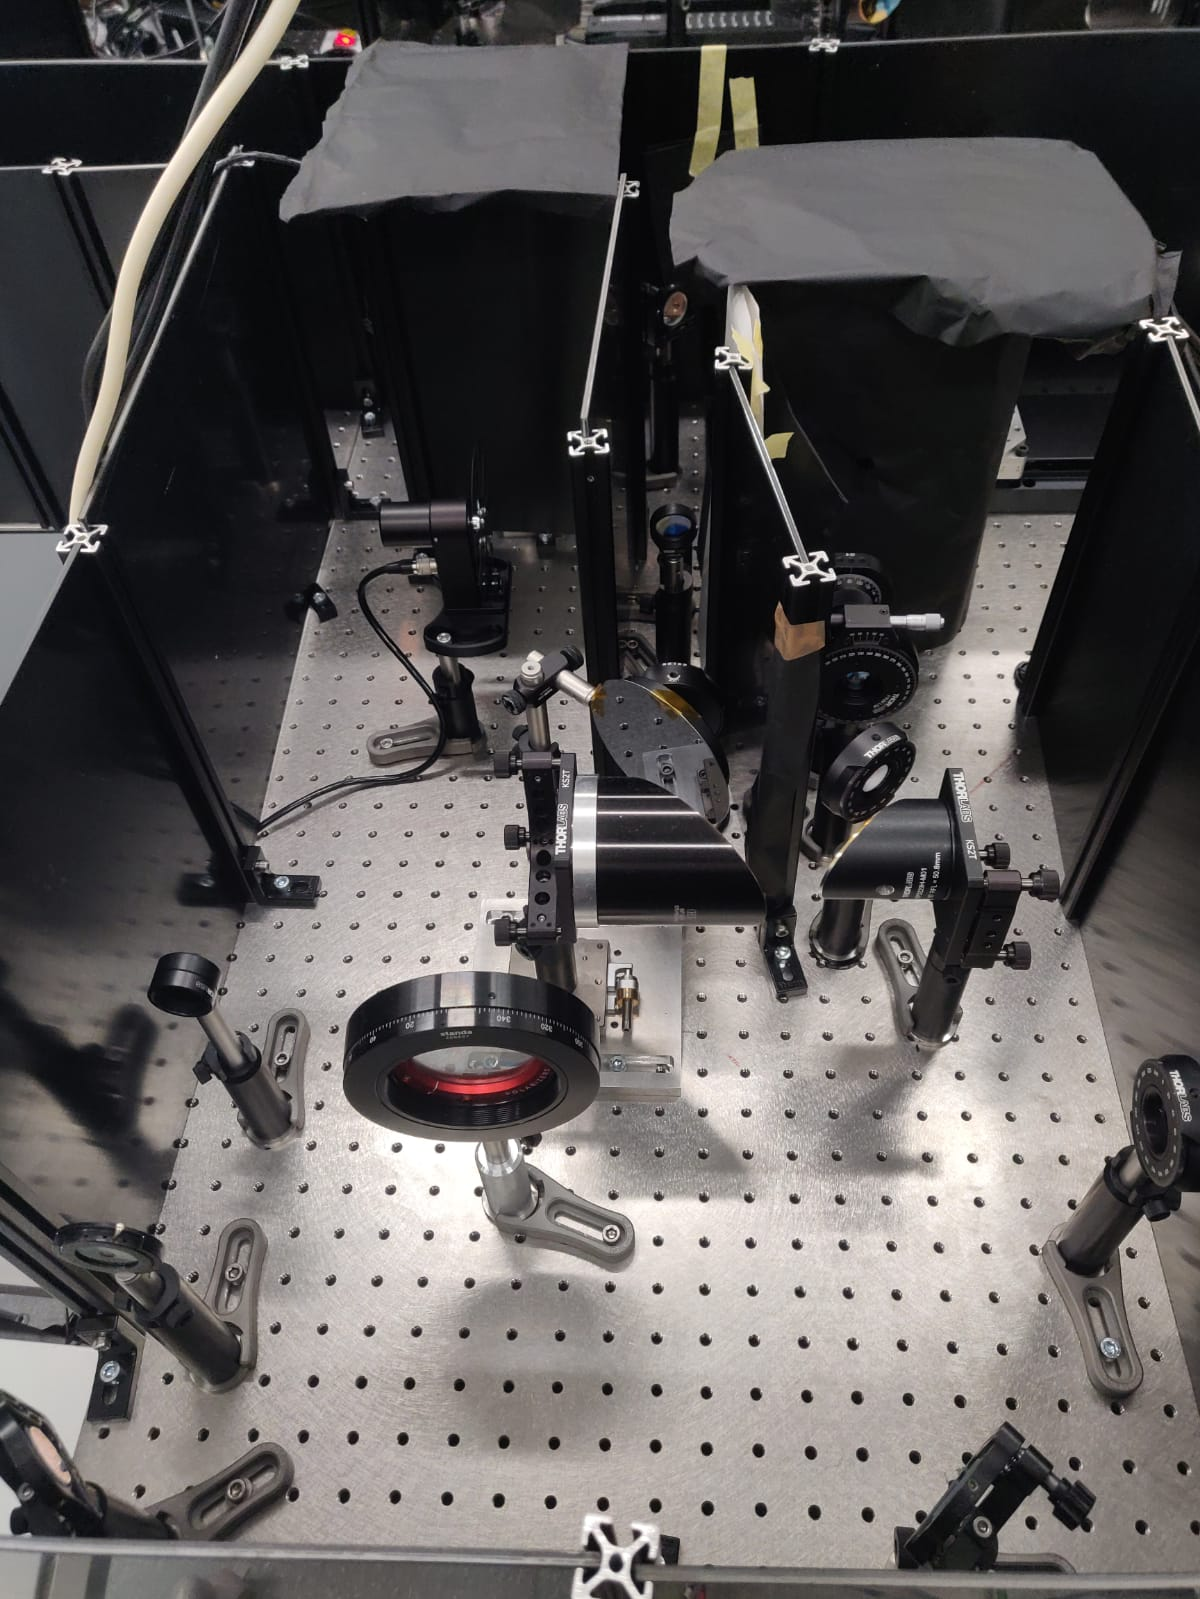
\includegraphics[width=0.2\textwidth]{images/setup.jpeg}}


\begin{document}

\maketitle

\section{Intro}

\begin{frame}{The Gap}
  \subsection{The spectrum}
  \begin{center}
  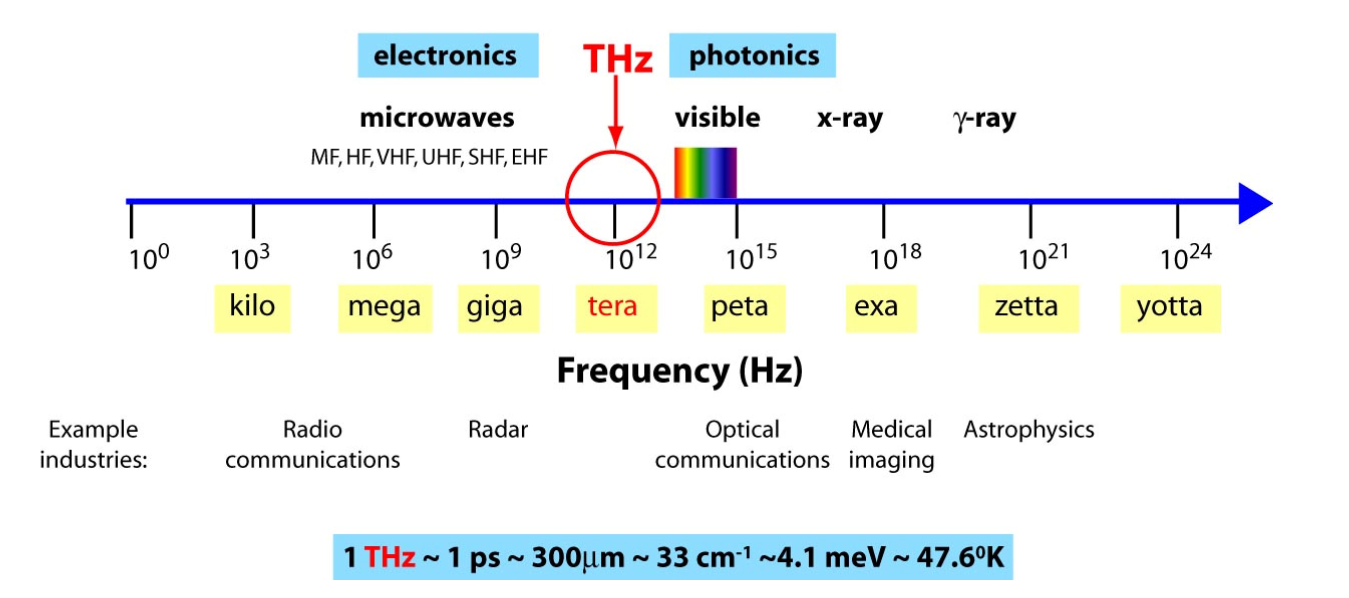
\includegraphics[width=0.7\textwidth]{images/spectrum.png}
  \end{center}
\end{frame}


\begin{frame}{Terahertz}
  \subsection{Applications}
  So why do we need terahertz radiation?
  \begin{itemize}
    \item medicine
    \item security
    \item data transmission \& saving
    \item physics
  \end{itemize}
\end{frame}

\begin{frame}{Outline}
  \tableofcontents
\end{frame}

\section{Setup}

\begin{frame}{But how to produce THz?}
  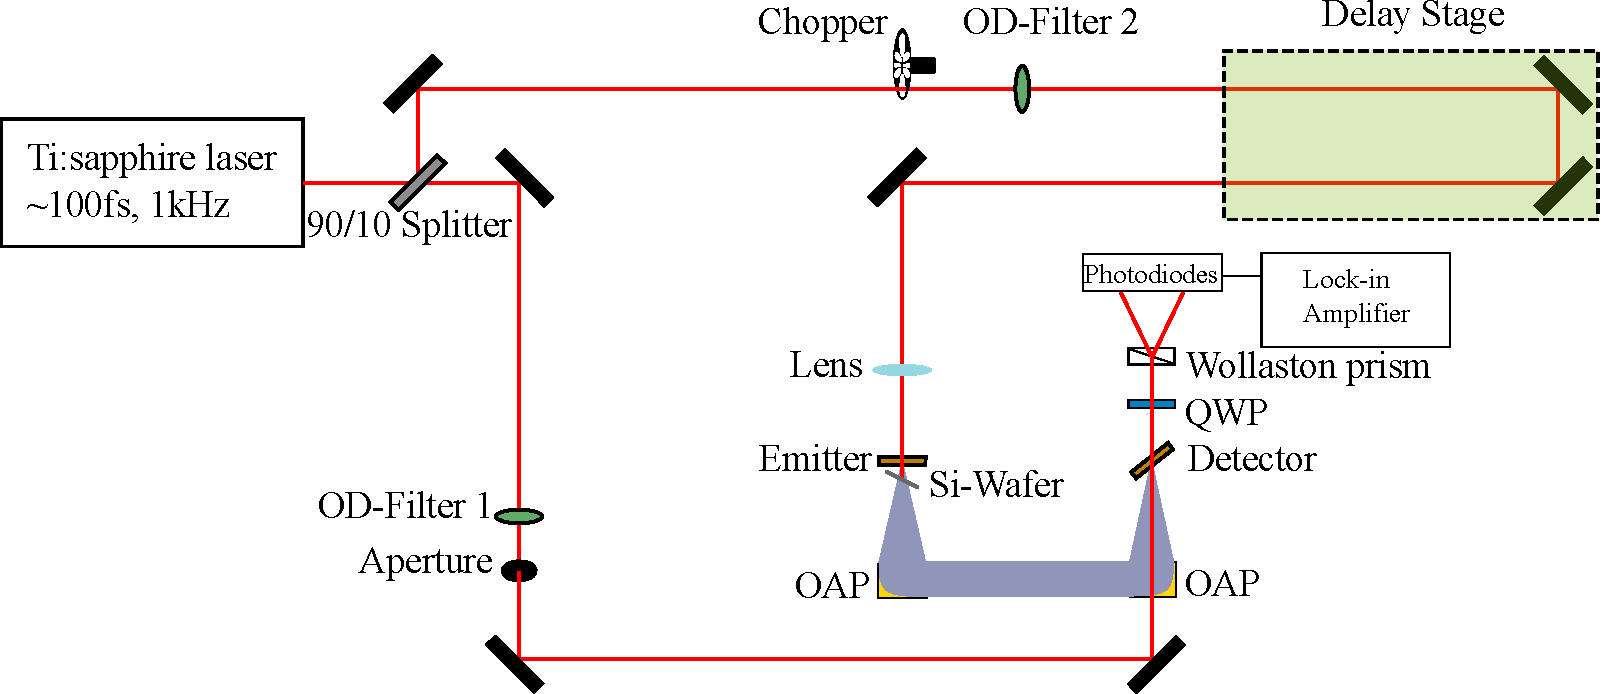
\includegraphics[width=\textwidth]{images/Aufbau.pdf}
\end{frame}

\section{Theory}
\subsection{Optical-rectification}
\begin{frame}{Optical-rectification}
 Polarisation
  \begin{align}
    \frac{P}{\epsilon_0} =& \chi_1E + \chi_2 E^2 + \chi_3 E^3 + ... \\
    \frac{P_\text{nl}}{\epsilon_0} =& \chi_2 \frac{E_0^2}{2} \left[ \cos((\omega_\text{i} - \omega_\text{j})t) + \cos((\omega_\text{i} + \omega_\text{j})t) \right ]
  \end{align}
  Energy conservation
  \begin{columns}
    \begin{column}{.4\textwidth}
      \begin{itemize}
        \item Two photons go in
        \item Higher energy level
        \item two photon emission 
        \item energy drops to gorundstate
      \end{itemize}
    \end{column}
    \begin{column}{.5\textwidth}
      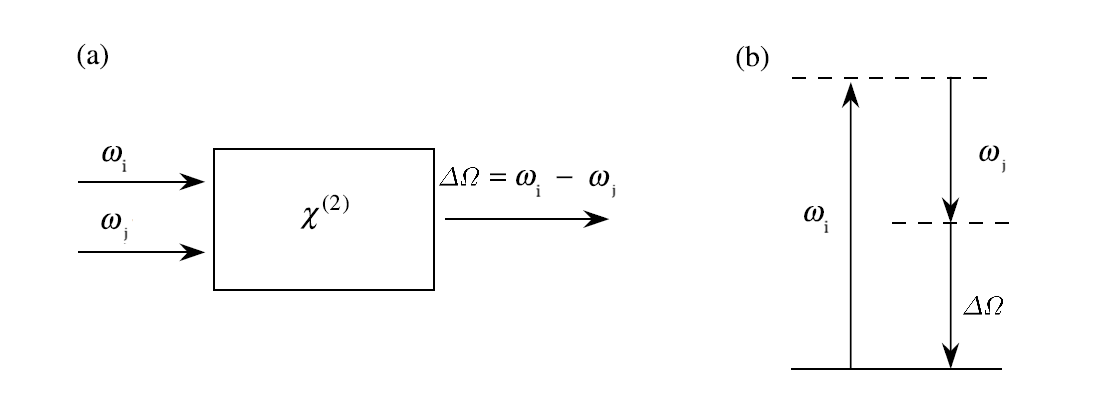
\includegraphics[width=\textwidth]{images/diffrence_frequency_mixing.PNG}
    \end{column}
  \end{columns}
\end{frame}
\subsection{Electro-optic sampling}
\begin{frame}{Electro-optic sampling (EOS)}
  And how to detect it?\\
  \textbf{Pockels effect!}\cite{THZ_eltric_field}
  \begin{equation}
    \frac{\symup{\Delta}I}{I} = \text{sin}(\theta) = \frac{2\pi}{\lambda} n_0^3 l r E_\text{THz}
\end{equation}
\begin{figure}
  \centering
  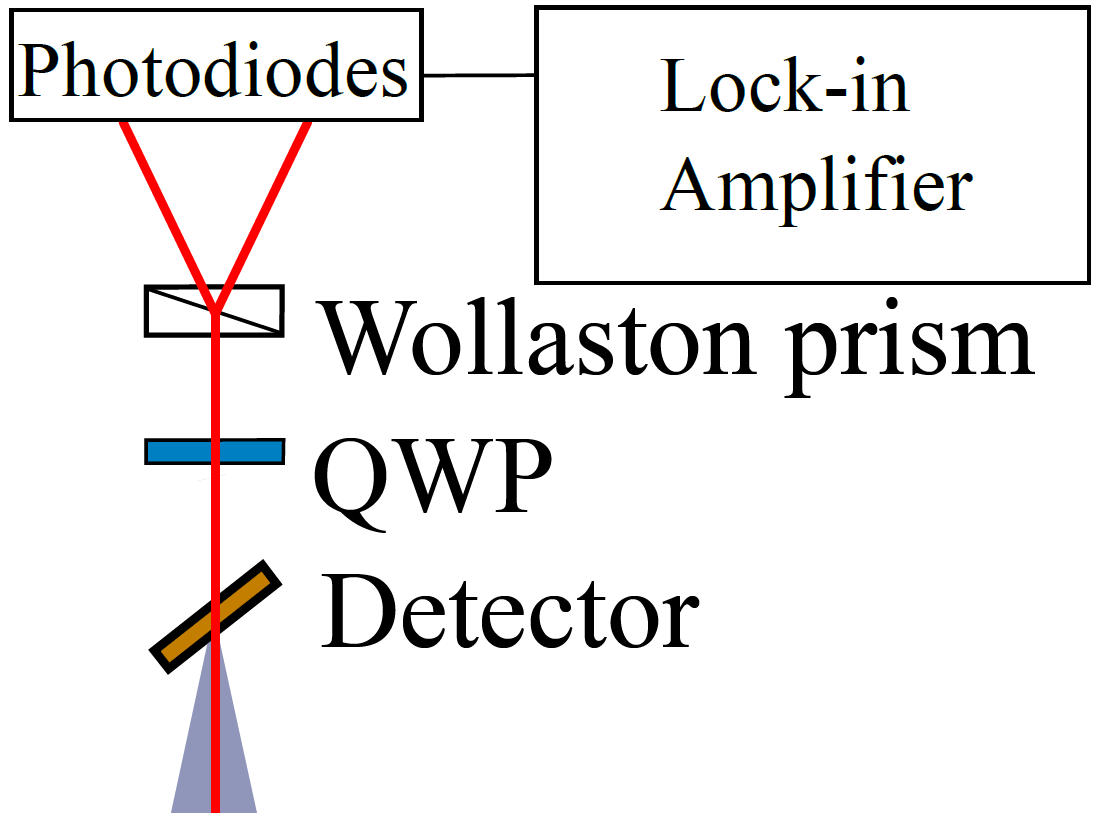
\includegraphics[width=0.5\textwidth]{images/detectionunit.png}
\end{figure}
\end{frame}

\subsection{Coherence-length}
\begin{frame}{Coherence-length}
\begin{equation}
    l(\omega_{\text{THz}}) = \frac{\pi c}{\omega_{\text{THz}} \left | n_\text{opt eff}(\omega_0) - n_{\text{THz}}(\omega_{\text{THz}})\right |}
\end{equation}
with 
\begin{equation}
    n_{\text{opt eff}} = n_\text{opt}(\omega) - \lambda_\text{opt}\frac{\partial n_\text{opt}}{\partial \lambda}\biggl{|}_{\lambda_\text{opt}}  
\end{equation}
\begin{center}
  \begin{columns}
    \begin{column}{.4\textwidth}
    \begin{figure}
      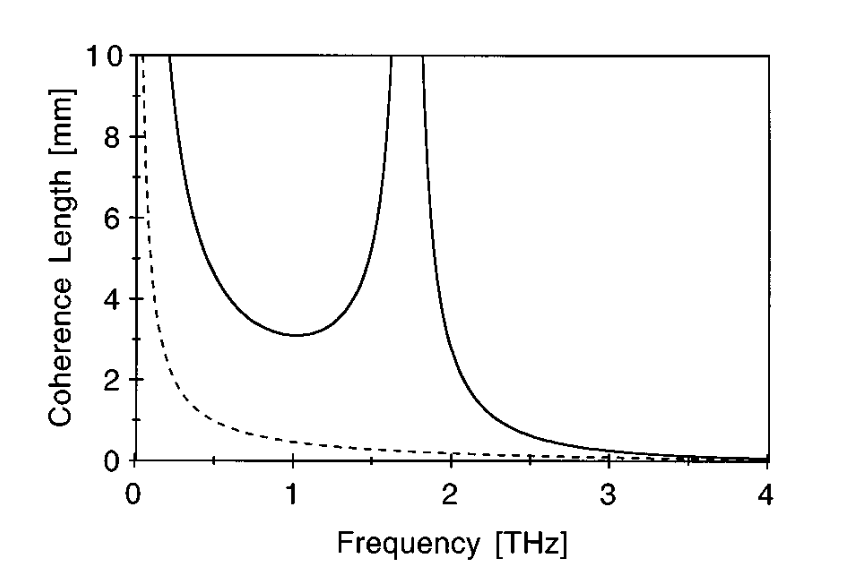
\includegraphics[width=0.9\textwidth]{images/coherence_length_ZnTe.png}
      \caption{(ZnTe) With $\SI{800}{\nano\meter}$ pump laser.}
    \end{figure}%
    \end{column}
    \begin{column}{.4\textwidth}
    \begin{figure}
      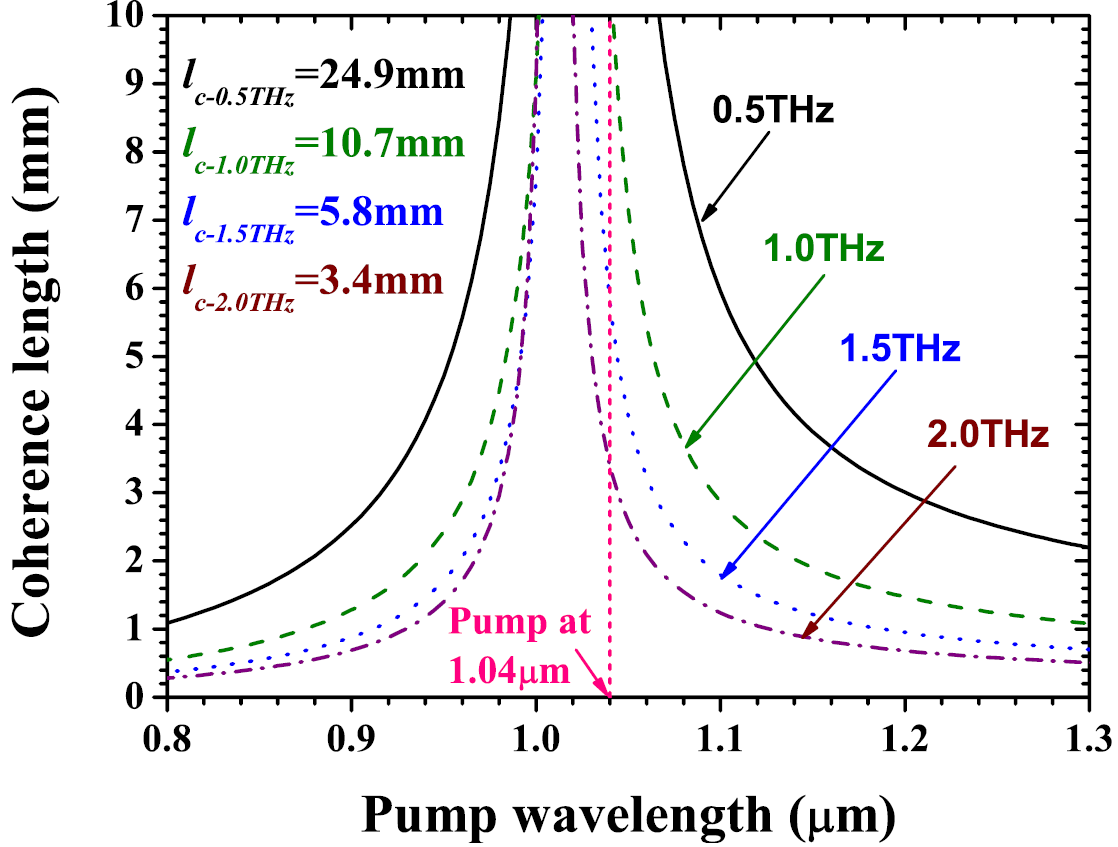
\includegraphics[width=0.8\textwidth]{images/GAP_coherencelength.png}
      \caption{(GaP) With various pump laser wavelengths.}
    \end{figure}
    \end{column}
  \end{columns}
\end{center}
\end{frame}

\section{Results}
\subsection{ZnTe}
\begin{frame}{EOS ZnTe}
\begin{figure}
  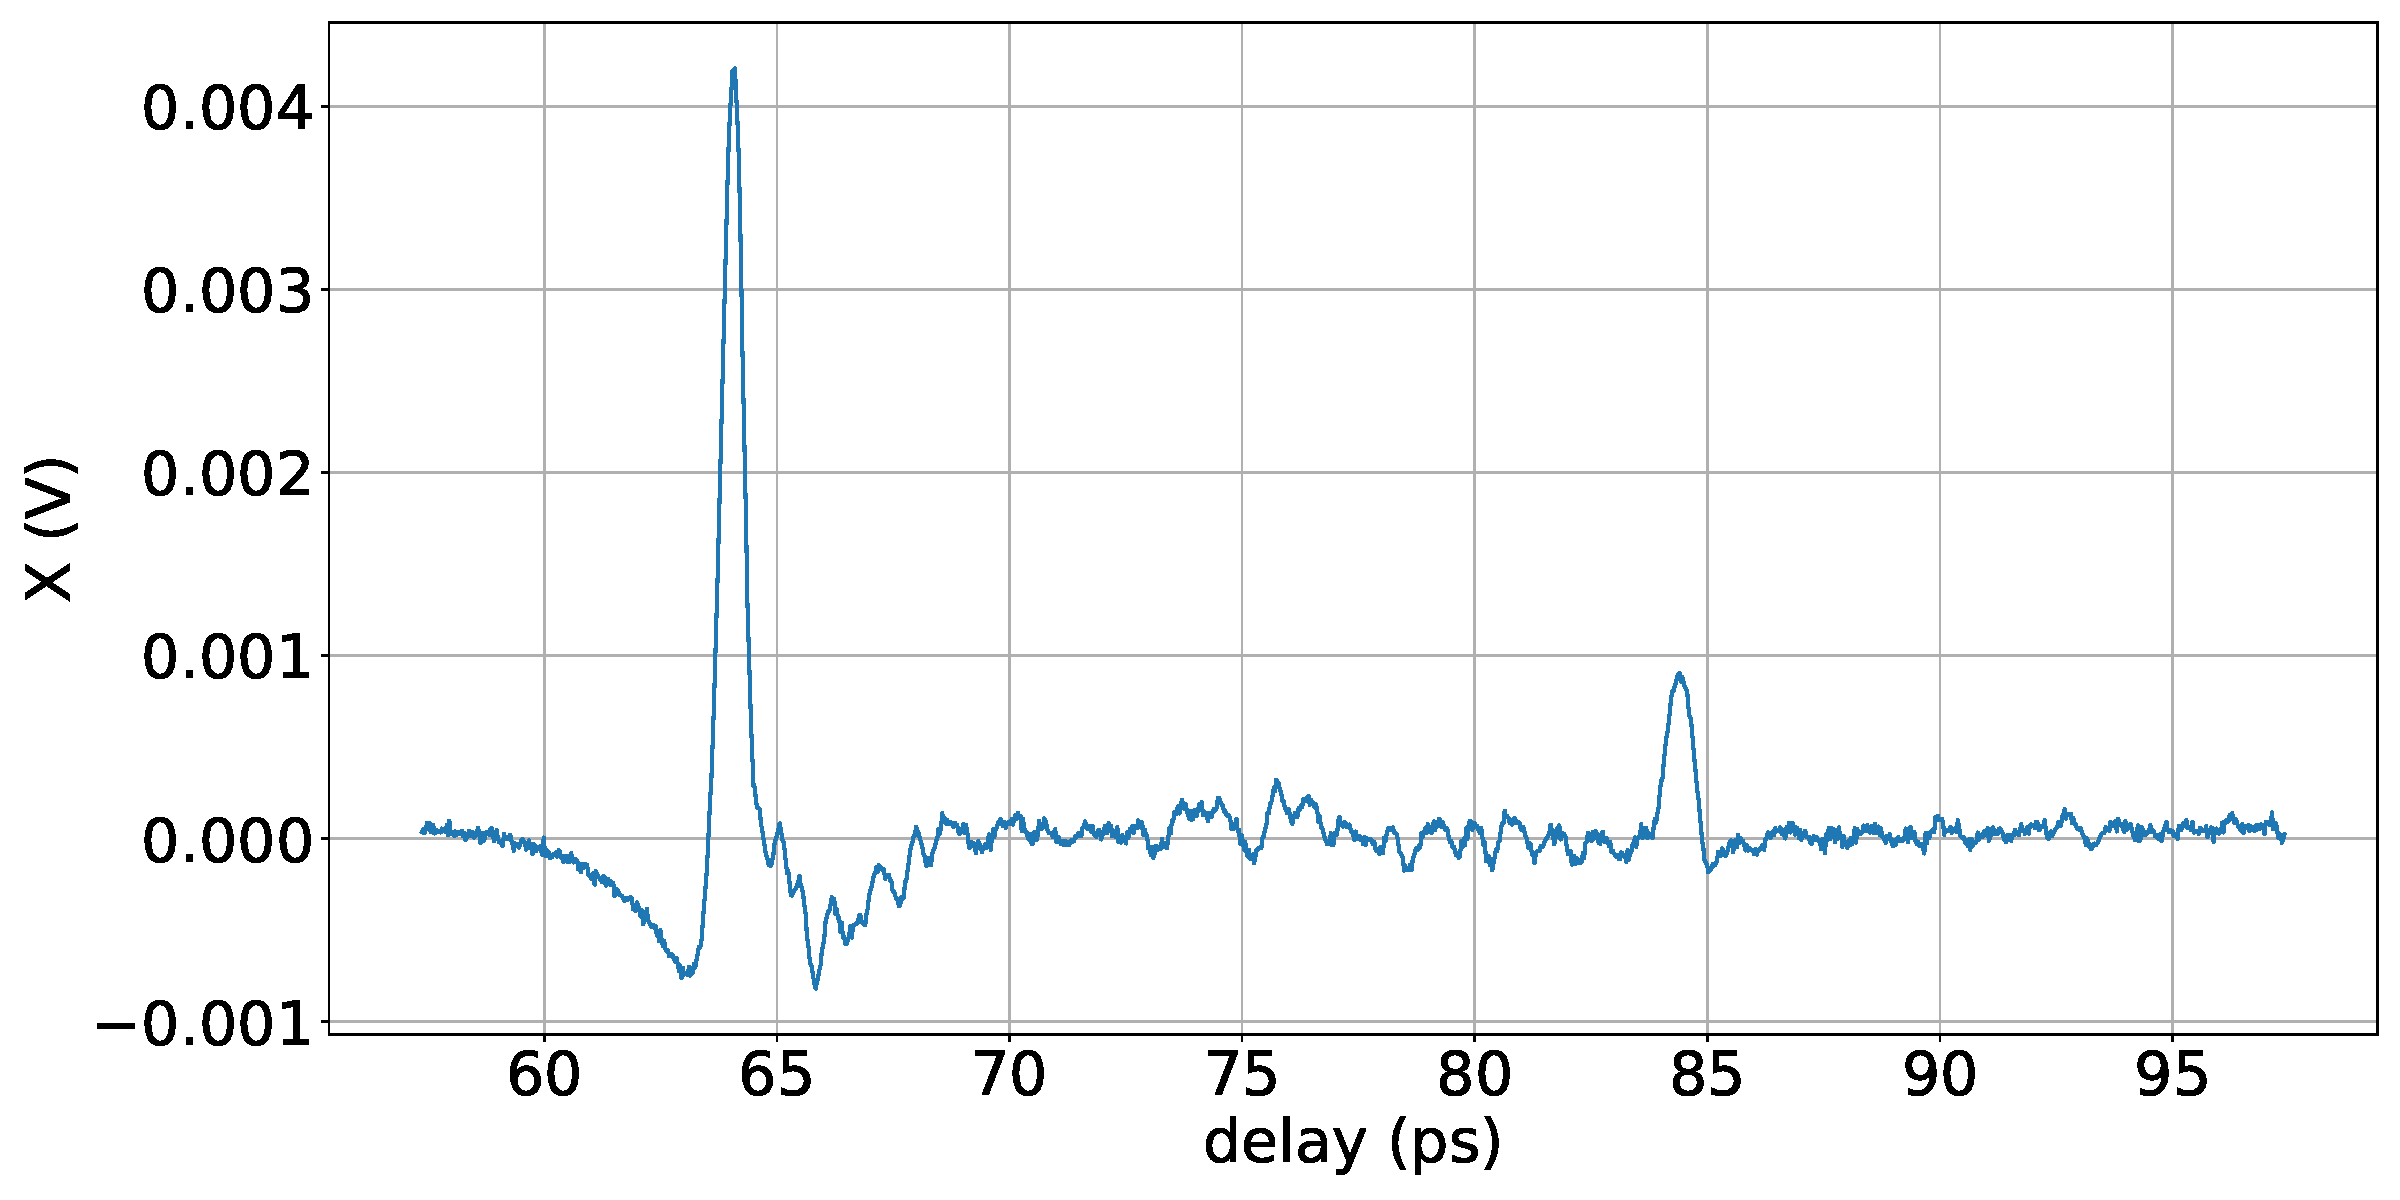
\includegraphics[width=0.8\textwidth]{images/2_11_30_20normalX.pdf}
\end{figure}
\end{frame}

\begin{frame}{Spectrum ZnTe}
  \begin{columns}
    \begin{column}{.5\textwidth}
  \begin{figure}
    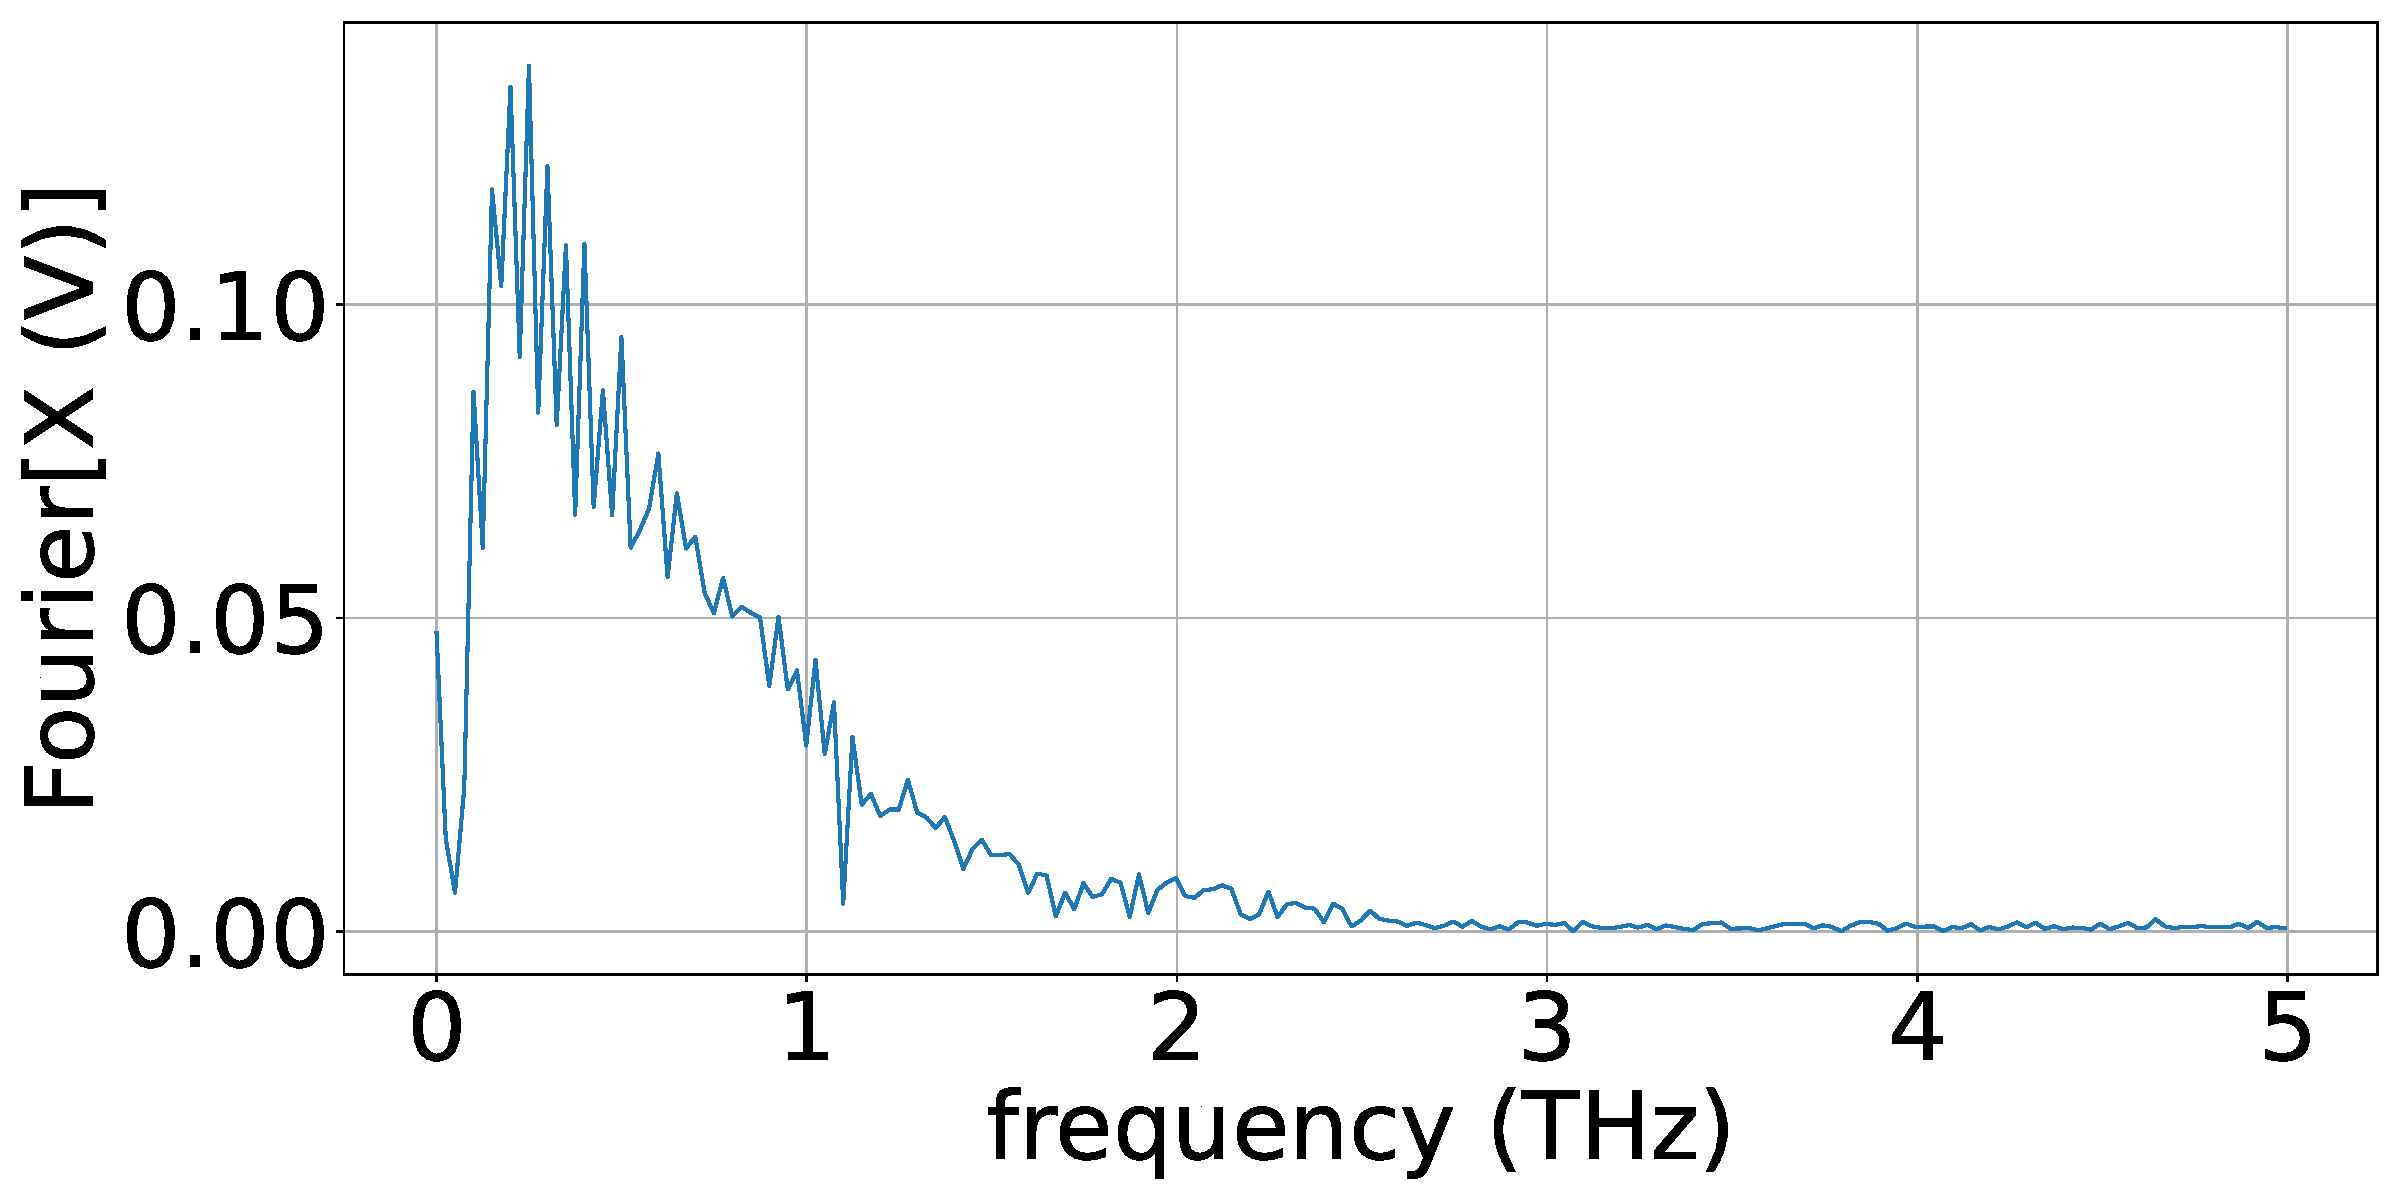
\includegraphics[width=\textwidth]{images/2_11_30_20normalFX.pdf}
    \caption{Spectrum ZnTe with $\SI{135.0}{\milli\W}$.}
  \end{figure}
  \end{column}
  \begin{column}{.5\textwidth}
    \begin{figure}
      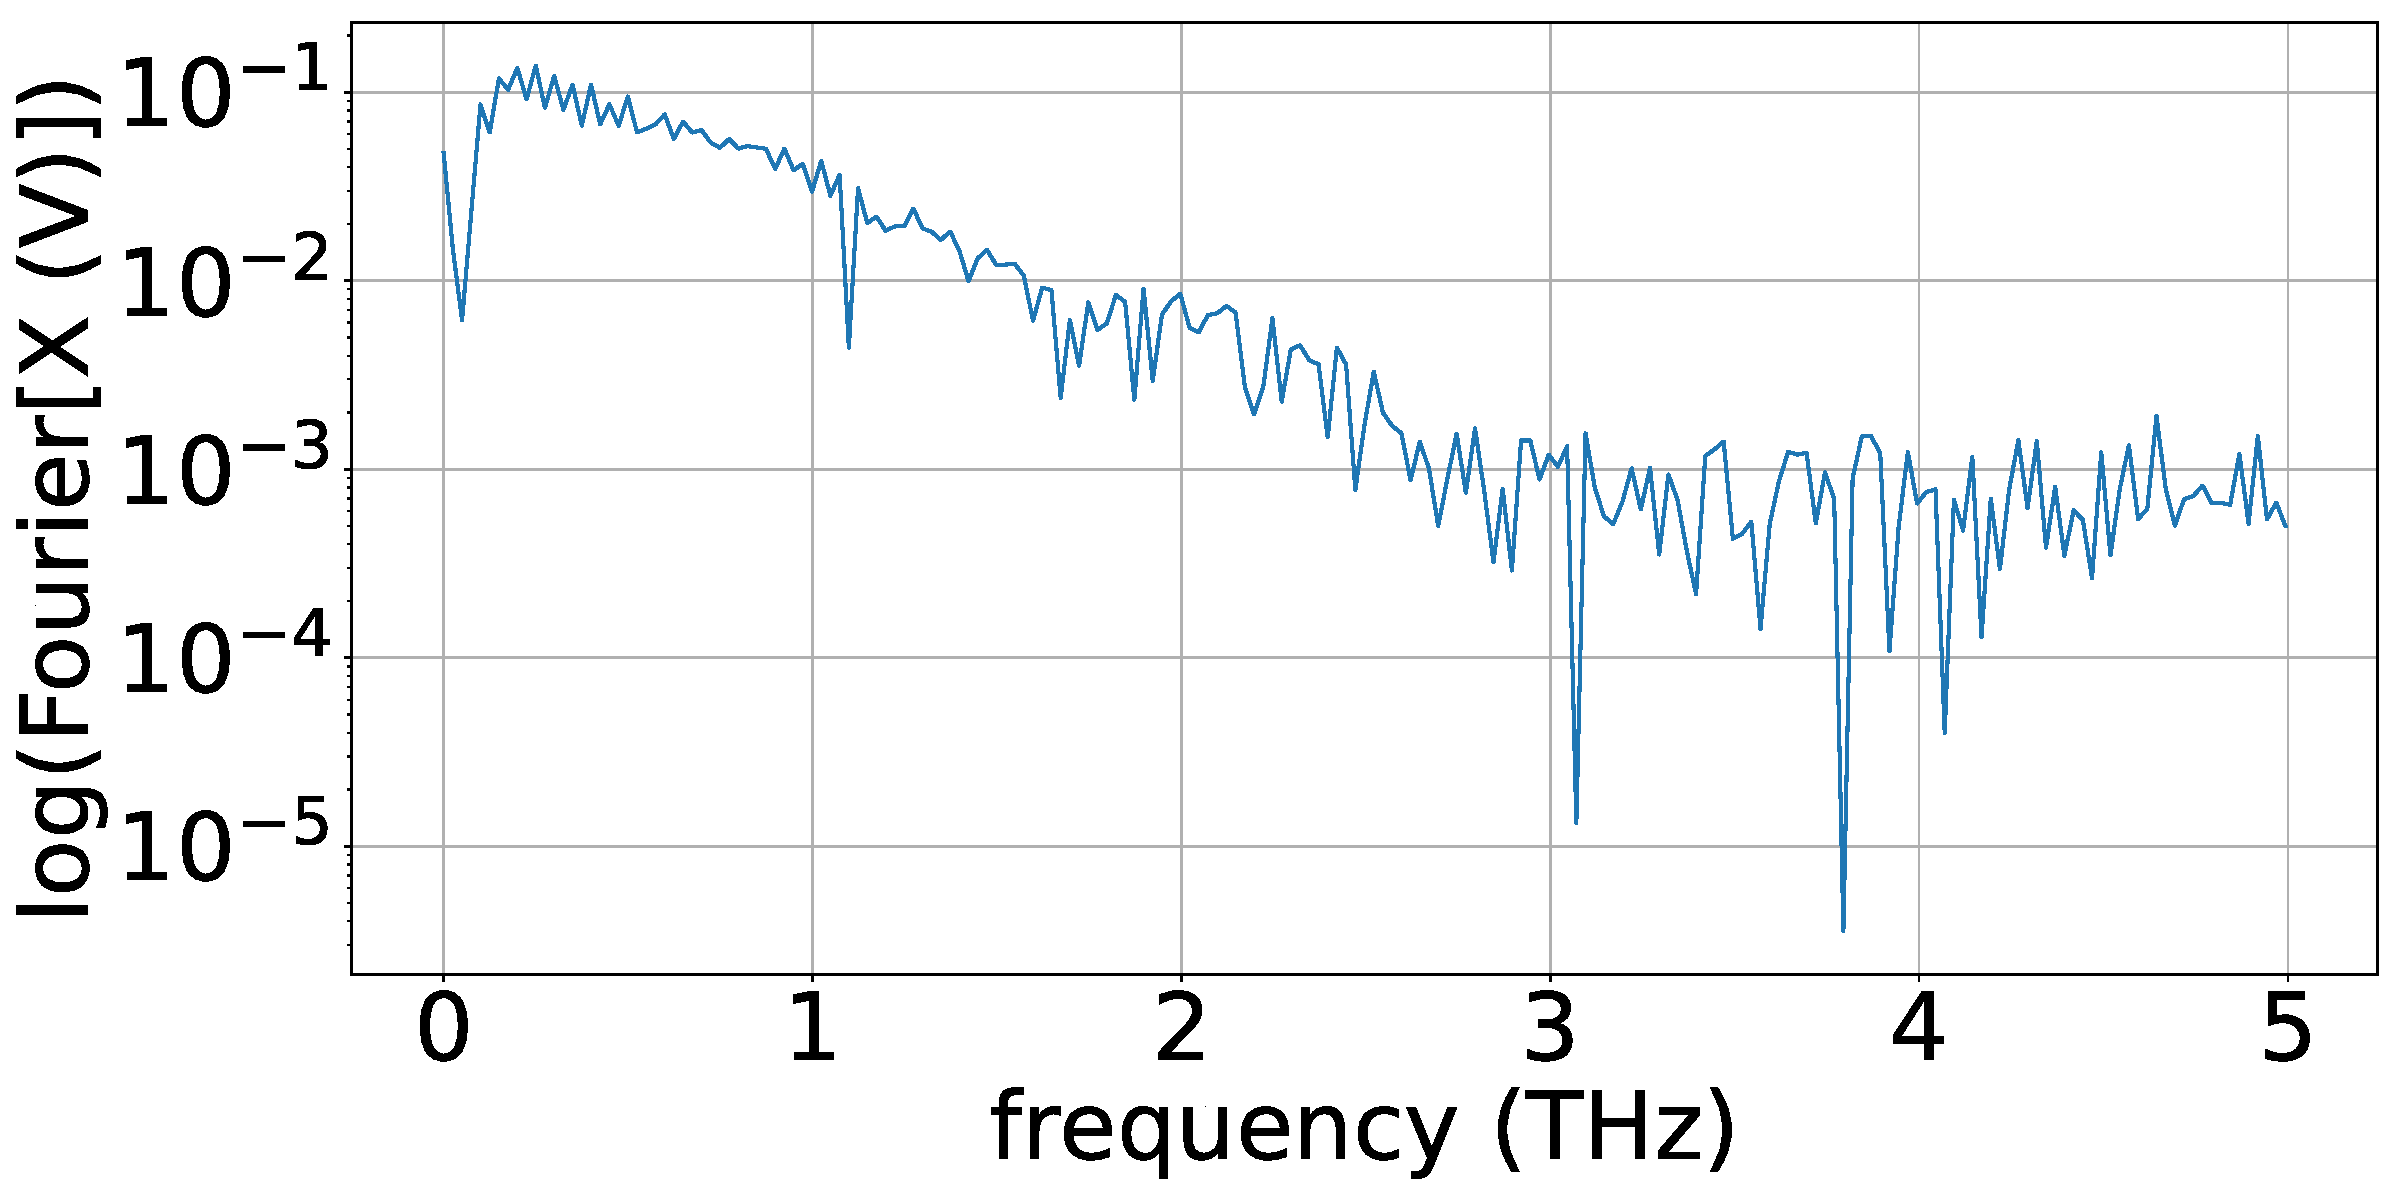
\includegraphics[width=\textwidth]{images/2_11_30_20normallog(FX).pdf}
      \caption{Spectrum ZnTe with $\SI{135.0}{\milli\W}$ with log y-axis.}
    \end{figure}    
  \end{column}
  \end{columns}
\end{frame}

\subsection{GaP}
\begin{frame}{EOS GaP}
  \begin{figure}
    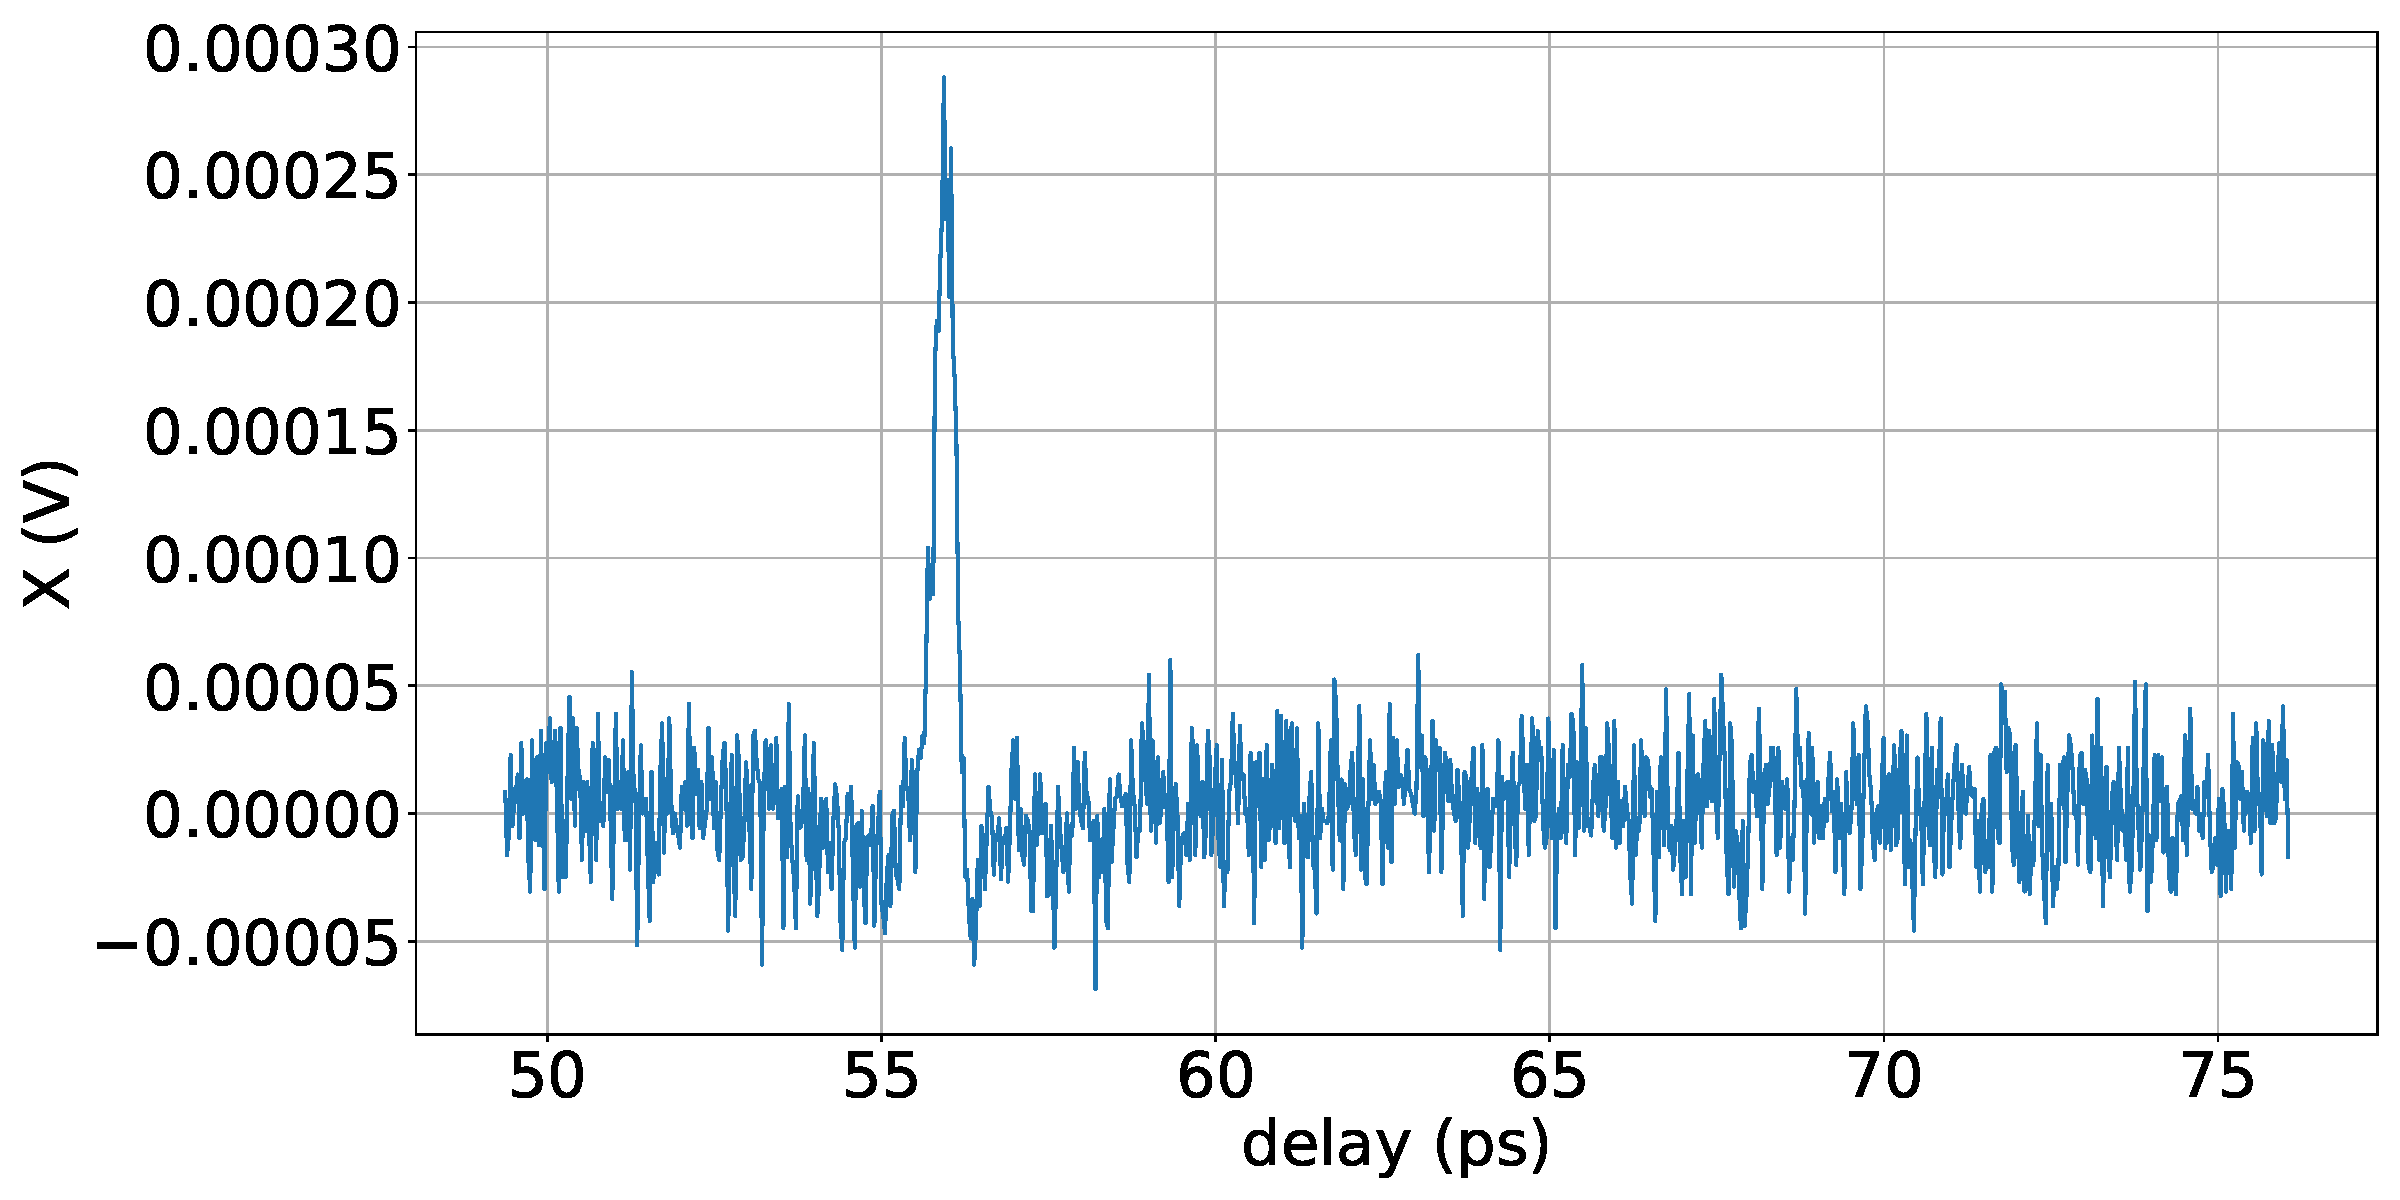
\includegraphics[width=0.8\textwidth]{images/GaP14_55_42normalX.pdf}
  \end{figure}
\end{frame}

\begin{frame}{Spectrum GaP}
  \begin{columns}
    \begin{column}{.5\textwidth}
  \begin{figure}
    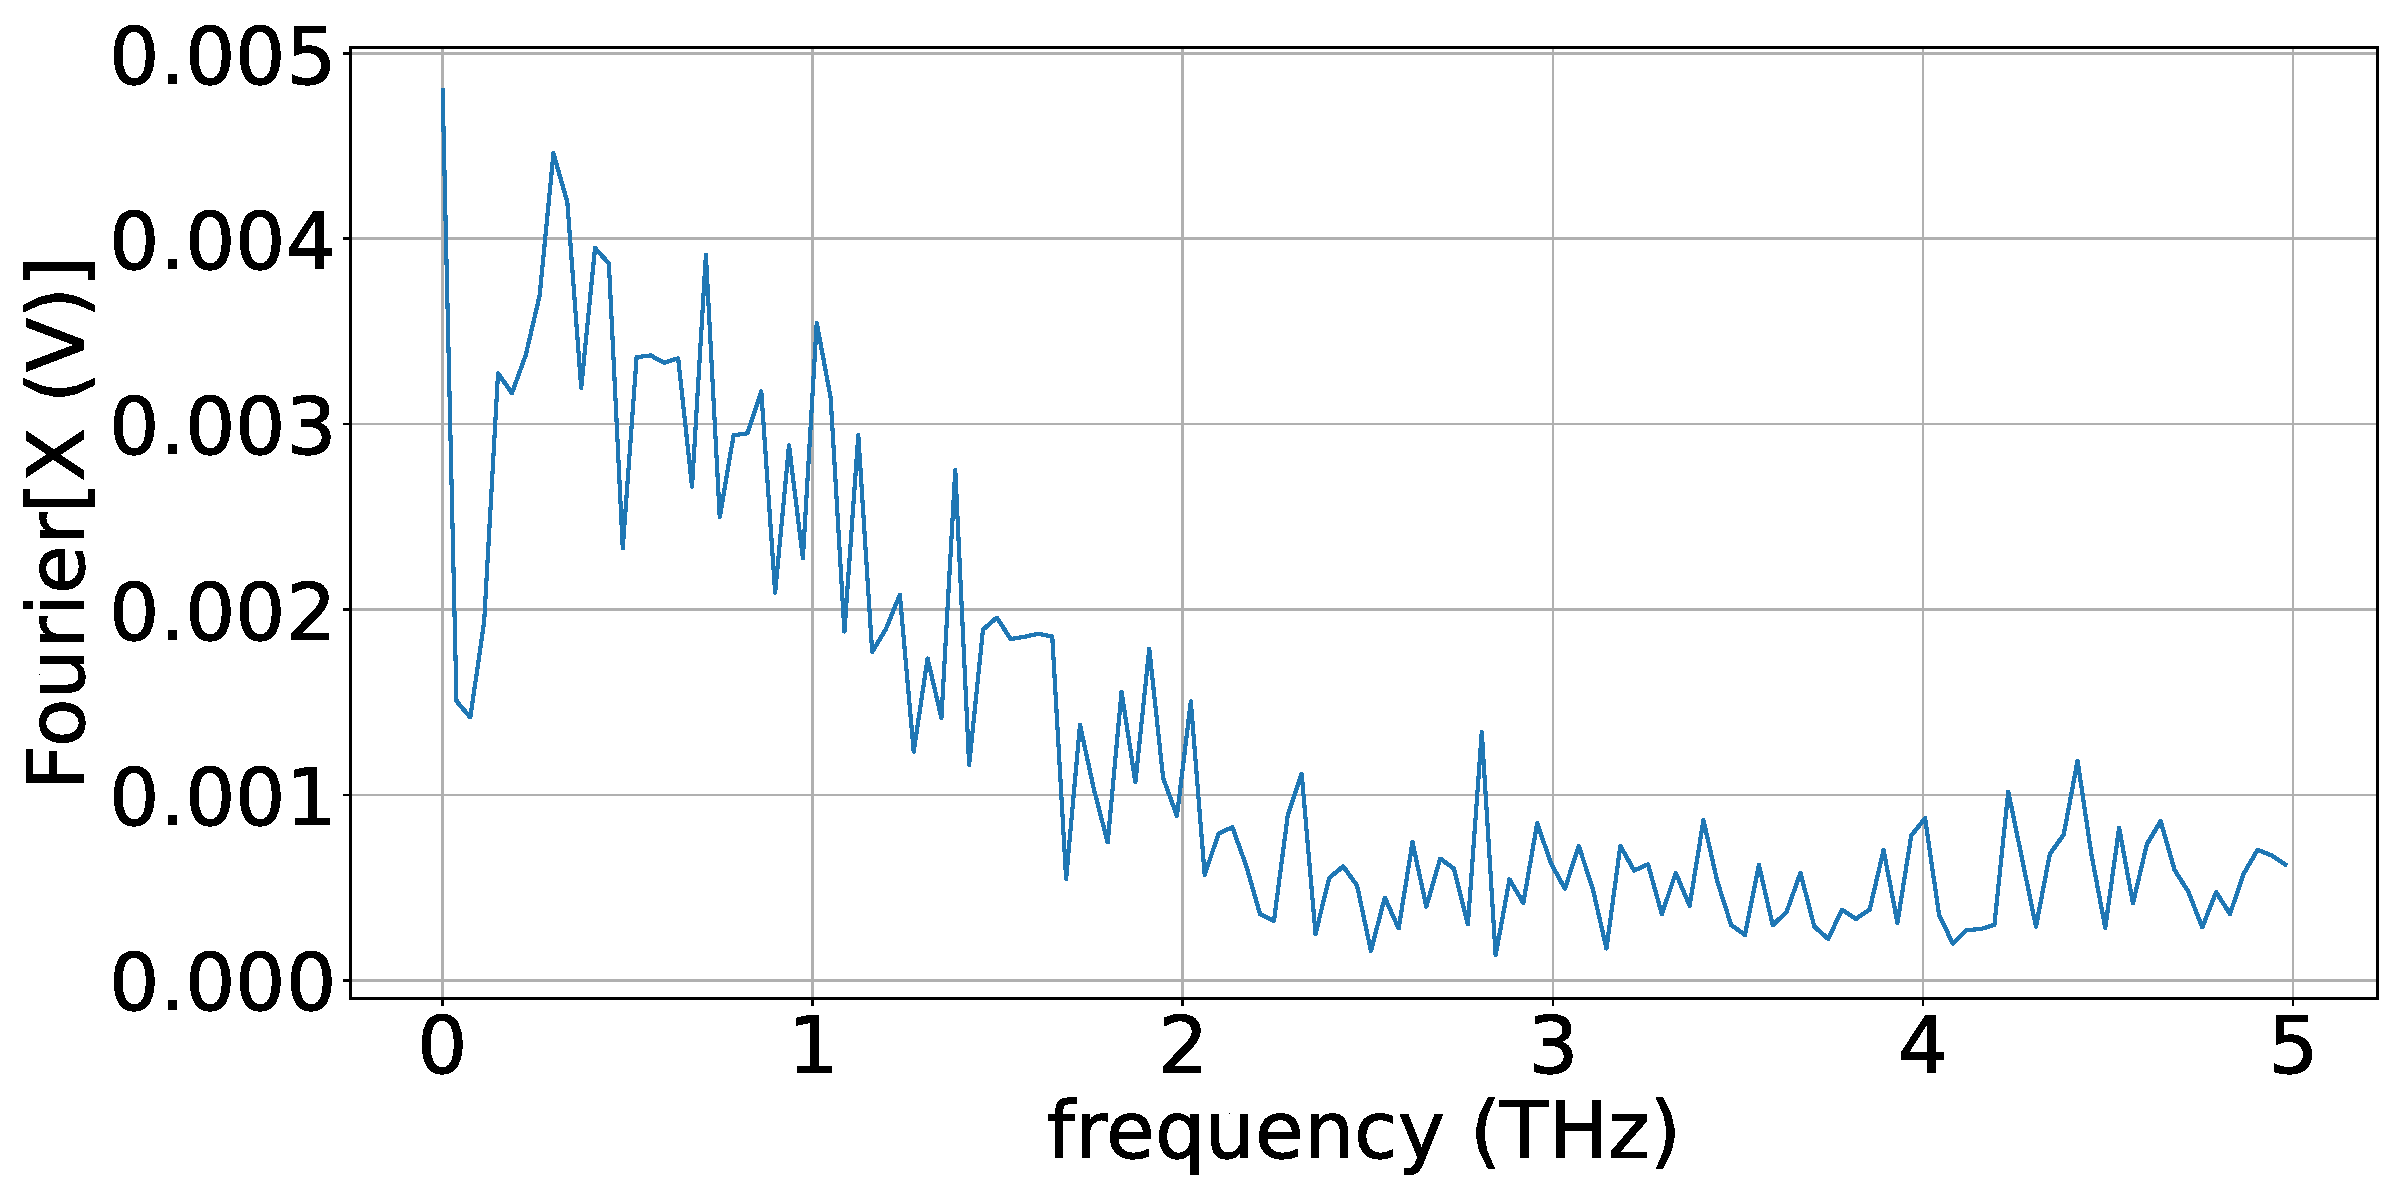
\includegraphics[width=\textwidth]{images/GaP14_55_42normalFX.pdf}
    \caption{Spectrum GaP with $\SI{124.2}{\milli\W}$.}
  \end{figure}
  \end{column}
  \begin{column}{.5\textwidth}
    \begin{figure}
      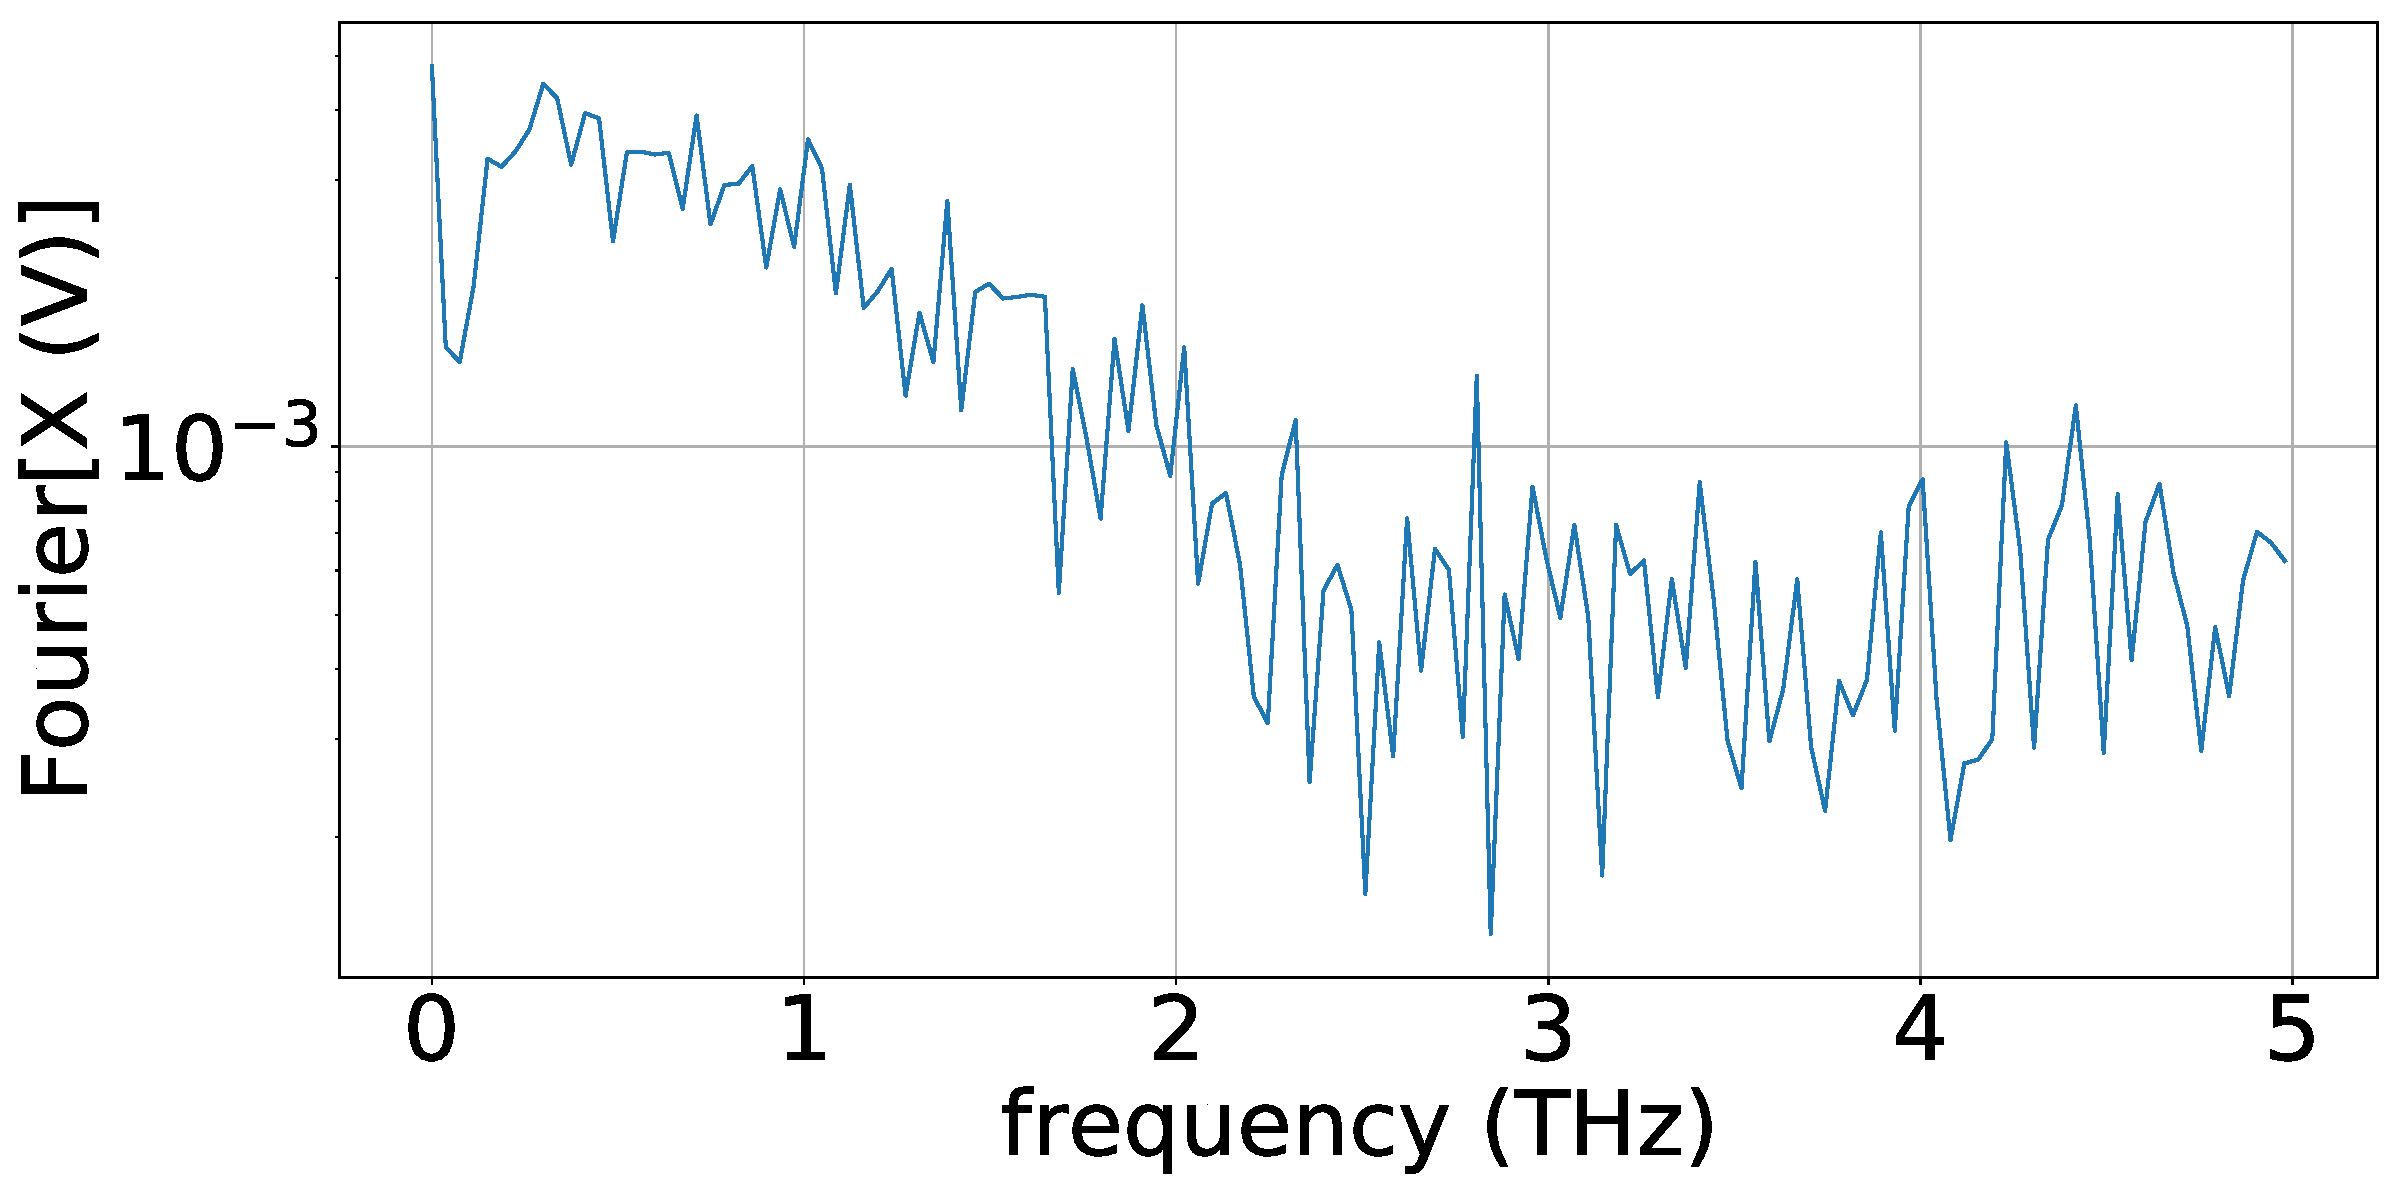
\includegraphics[width=\textwidth]{images/GaP14_55_42normallog(FX).pdf}
      \caption{Spectrum GaP with $\SI{124.2}{\milli\W}$ with log y-axis.}
    \end{figure}    
  \end{column}
  \end{columns}
\end{frame}

\subsection{Comparisson}

\begin{frame}{Spectra}
  \begin{columns}
    \begin{column}{.5\textwidth}
  \begin{figure}
    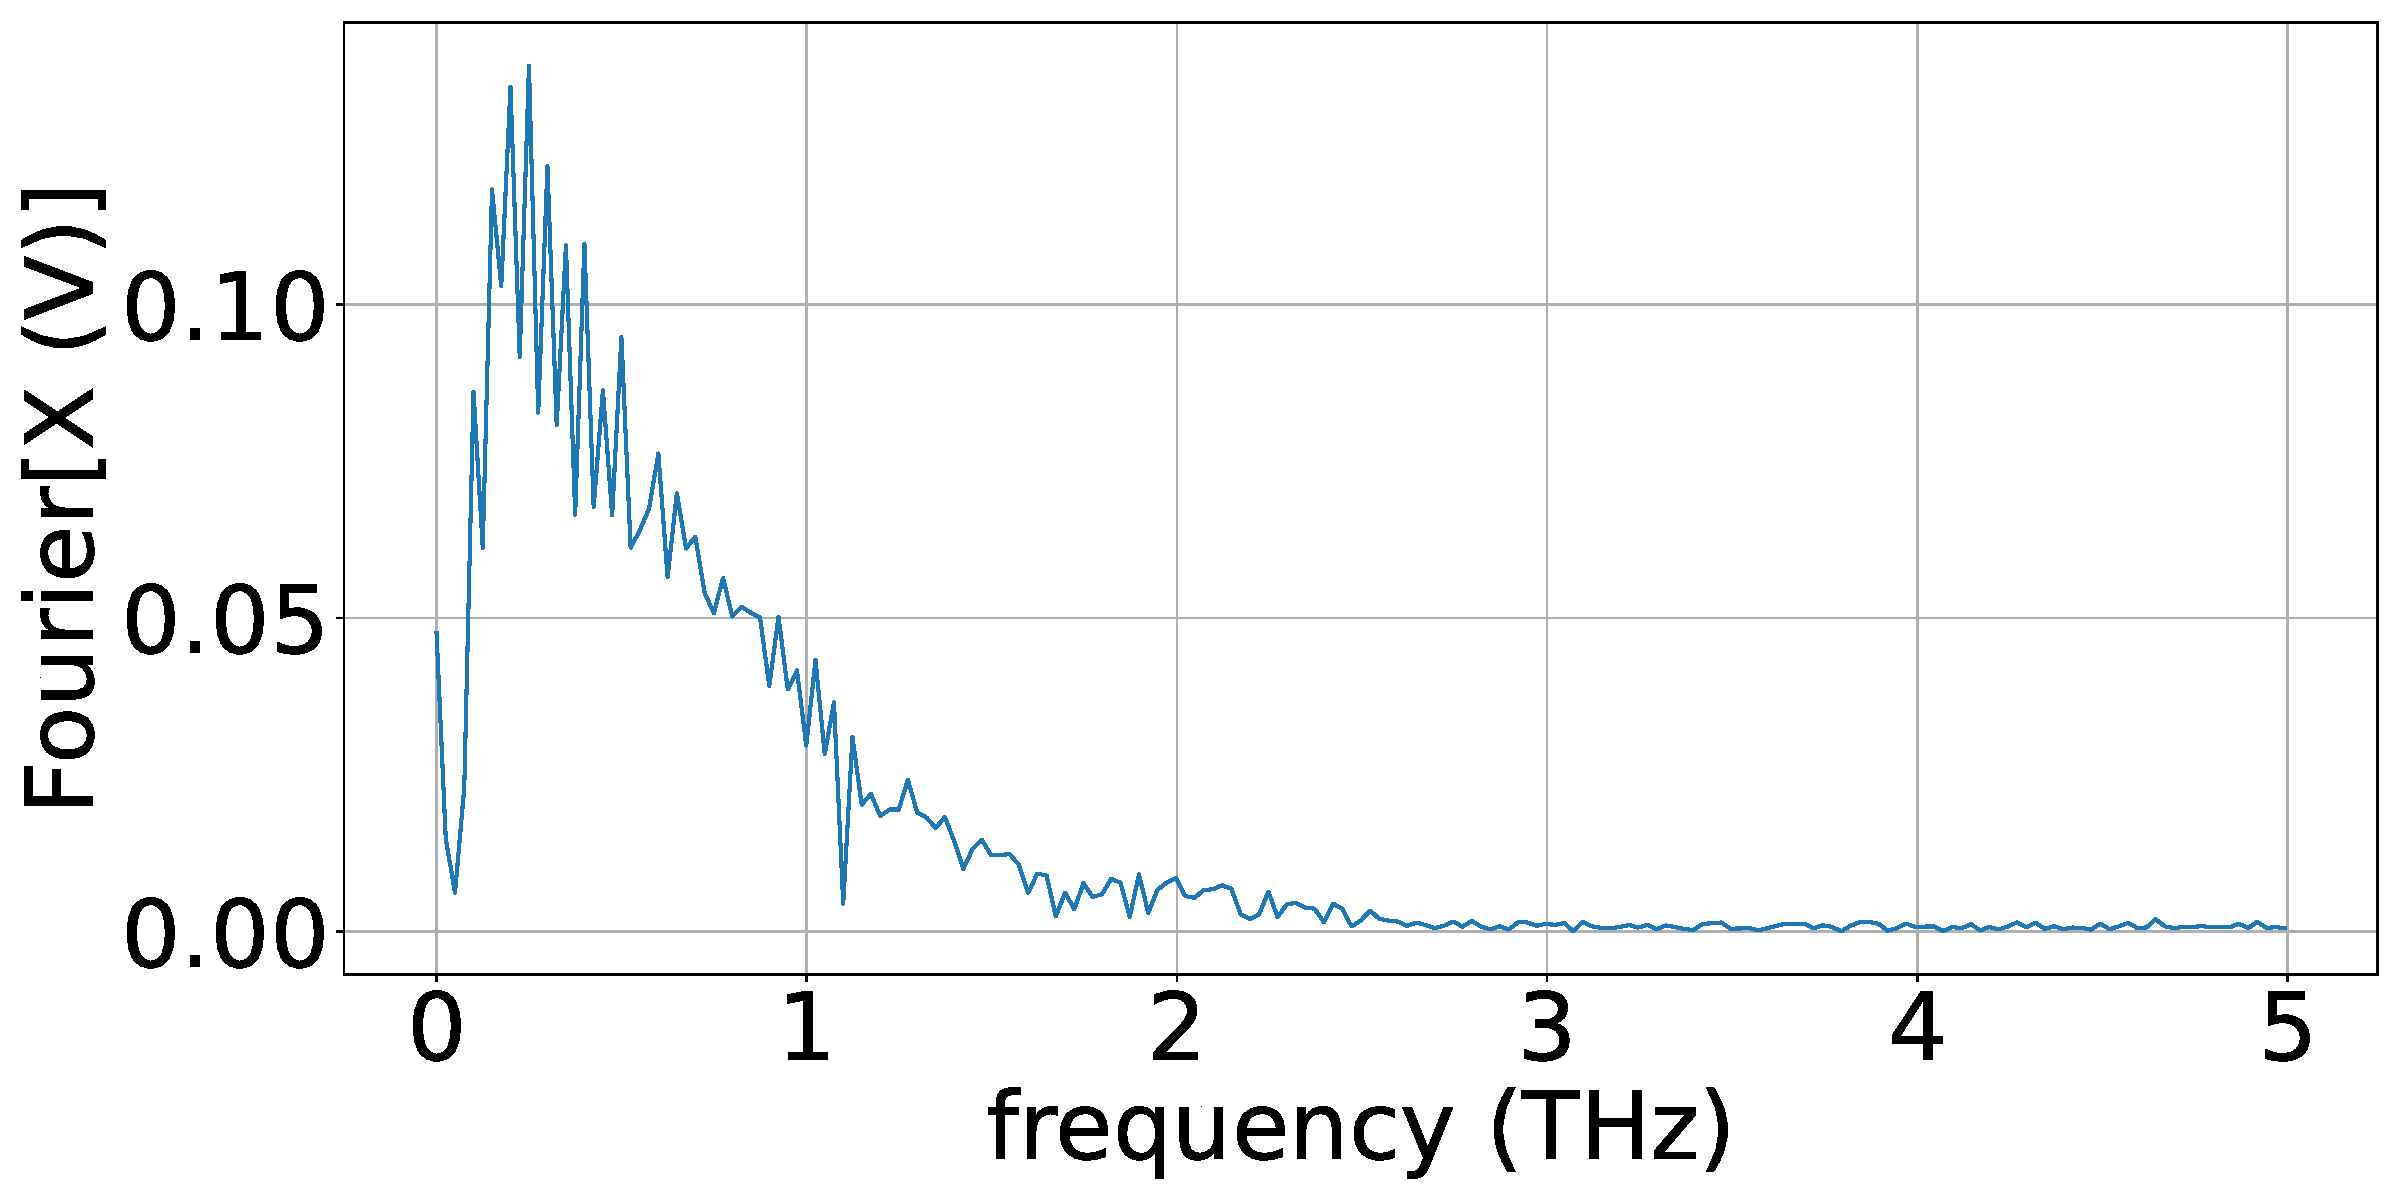
\includegraphics[width=\textwidth]{images/2_11_30_20normalFX.pdf}
    \caption{Spectrum of ZnTe with $\SI{135.0}{\milli\W}$ pump power.}
  \end{figure}
  \end{column}
  \begin{column}{.5\textwidth}
    \begin{figure}
      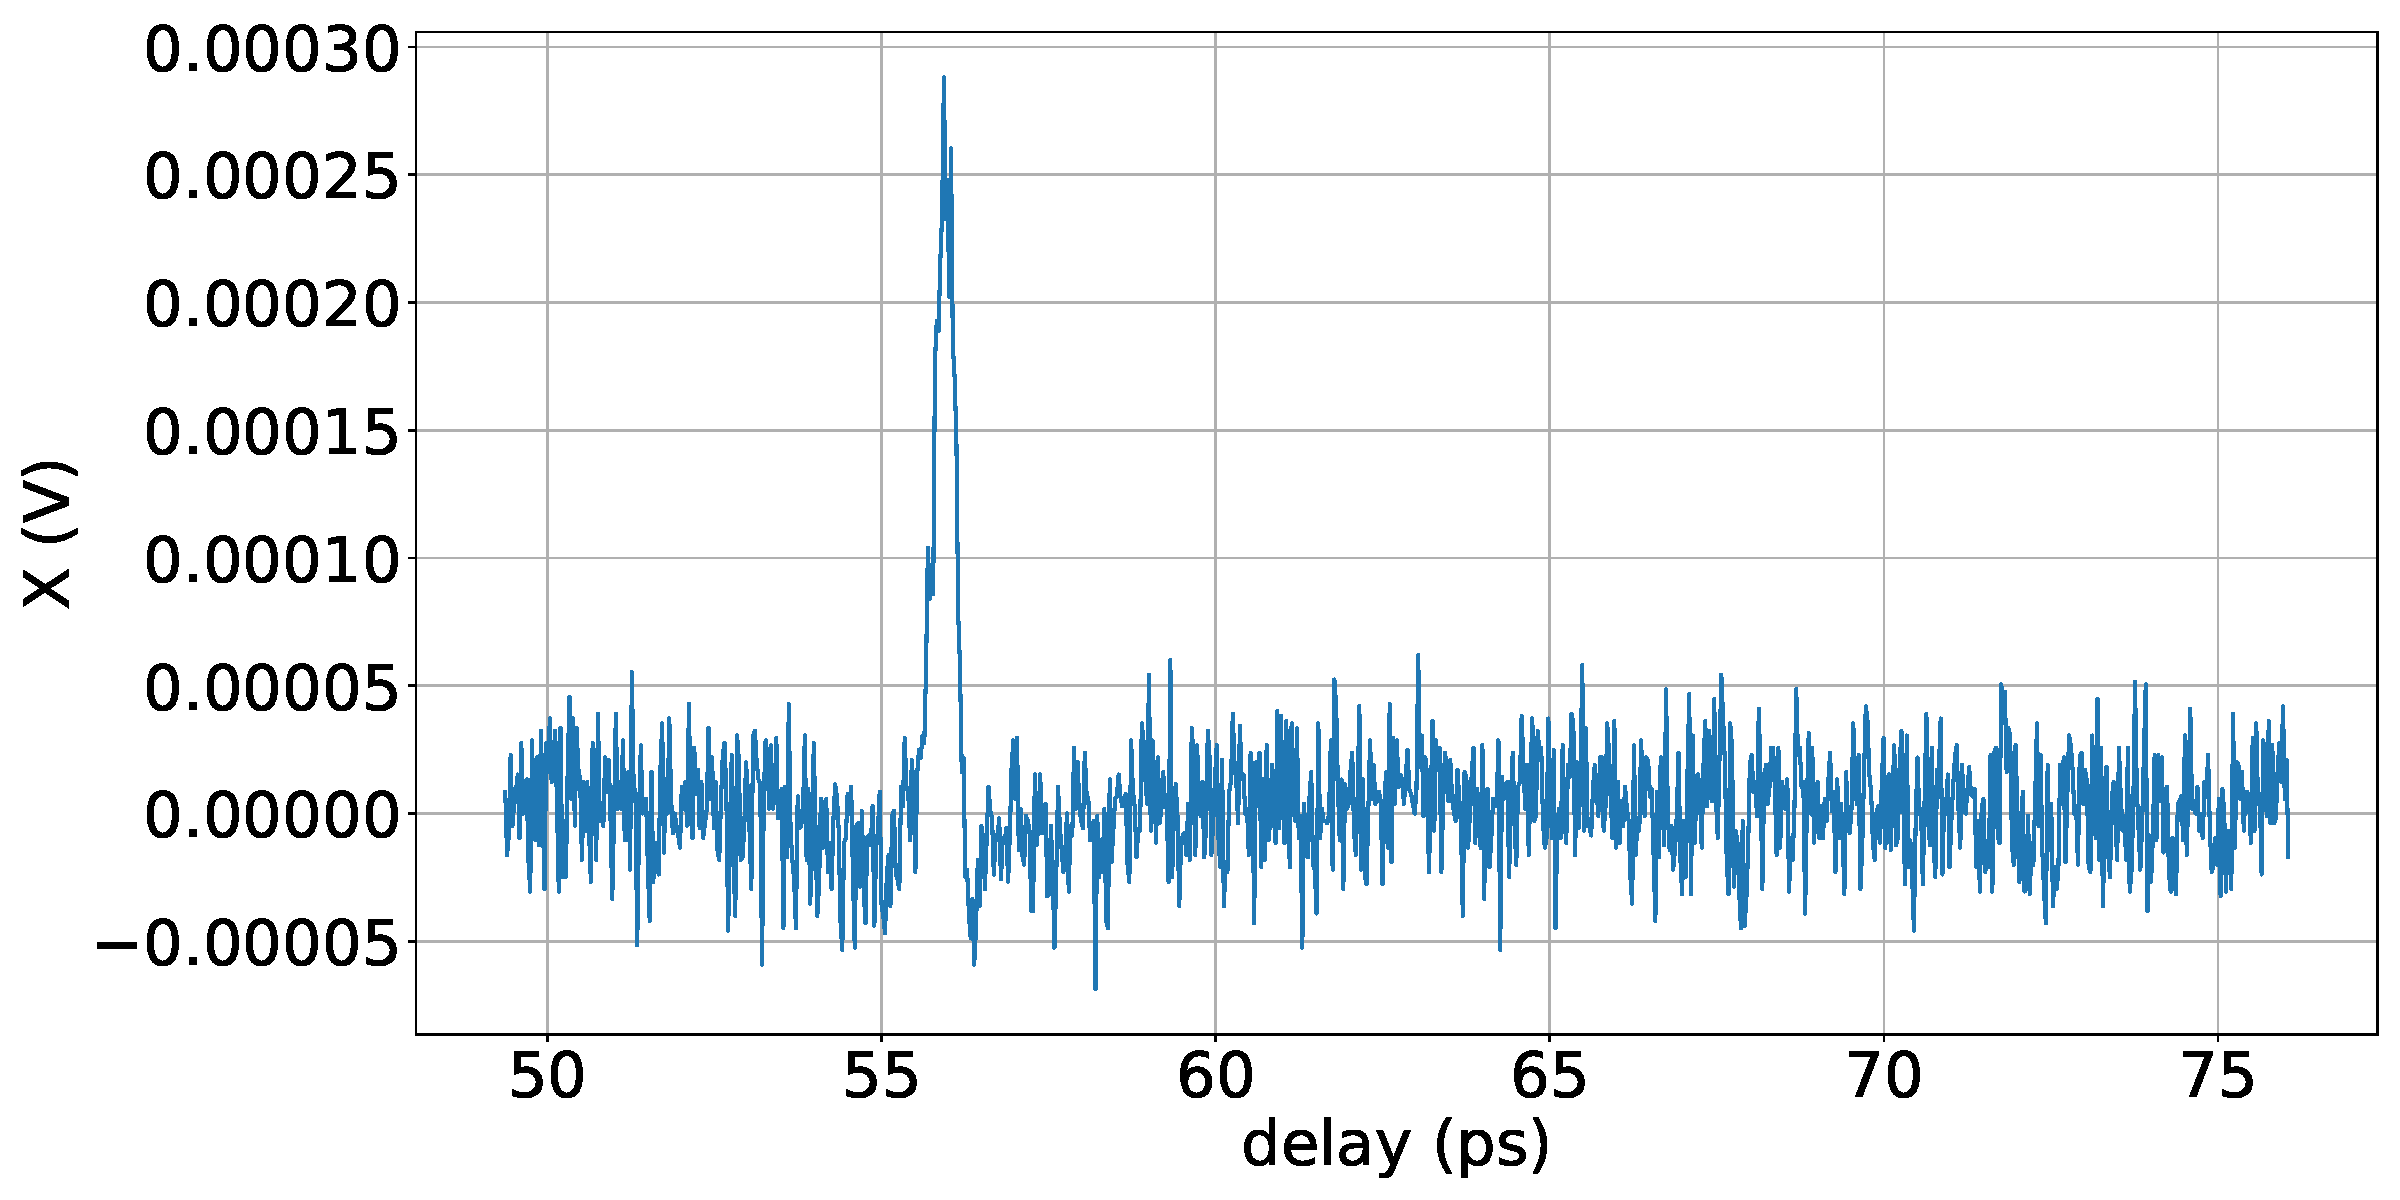
\includegraphics[width=\textwidth]{images/GaP14_55_42normalX.pdf}
      \caption{Spectrum GaP with $\SI{124.2}{\milli\W }$}
    \end{figure}    
  \end{column}
  \end{columns}
\end{frame}

\begin{frame}{Filter}
  Switch filter for different pump powers:
  \begin{figure}
    \begin{overprint}
      \onslide<1>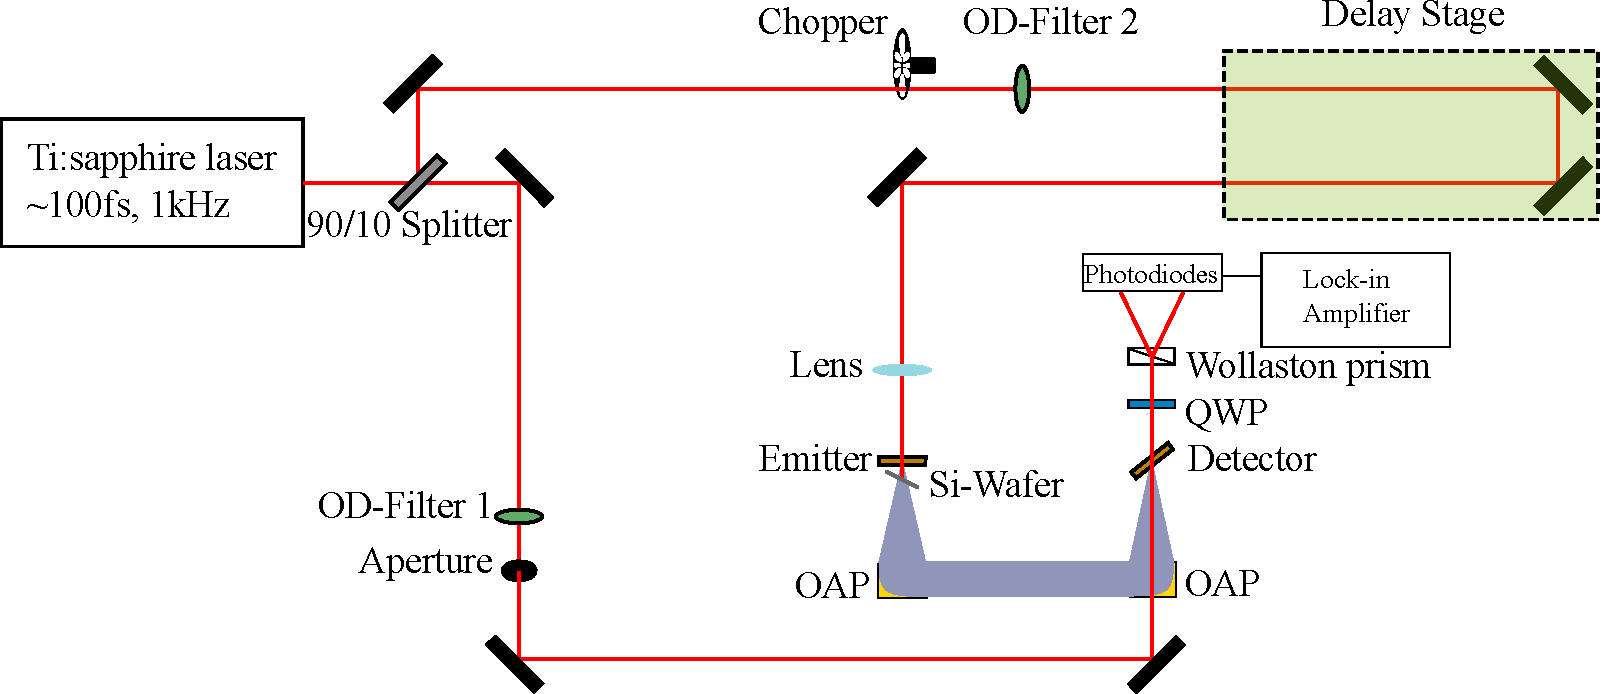
\includegraphics[width=\textwidth]{images/Aufbau.pdf}
      \onslide<2>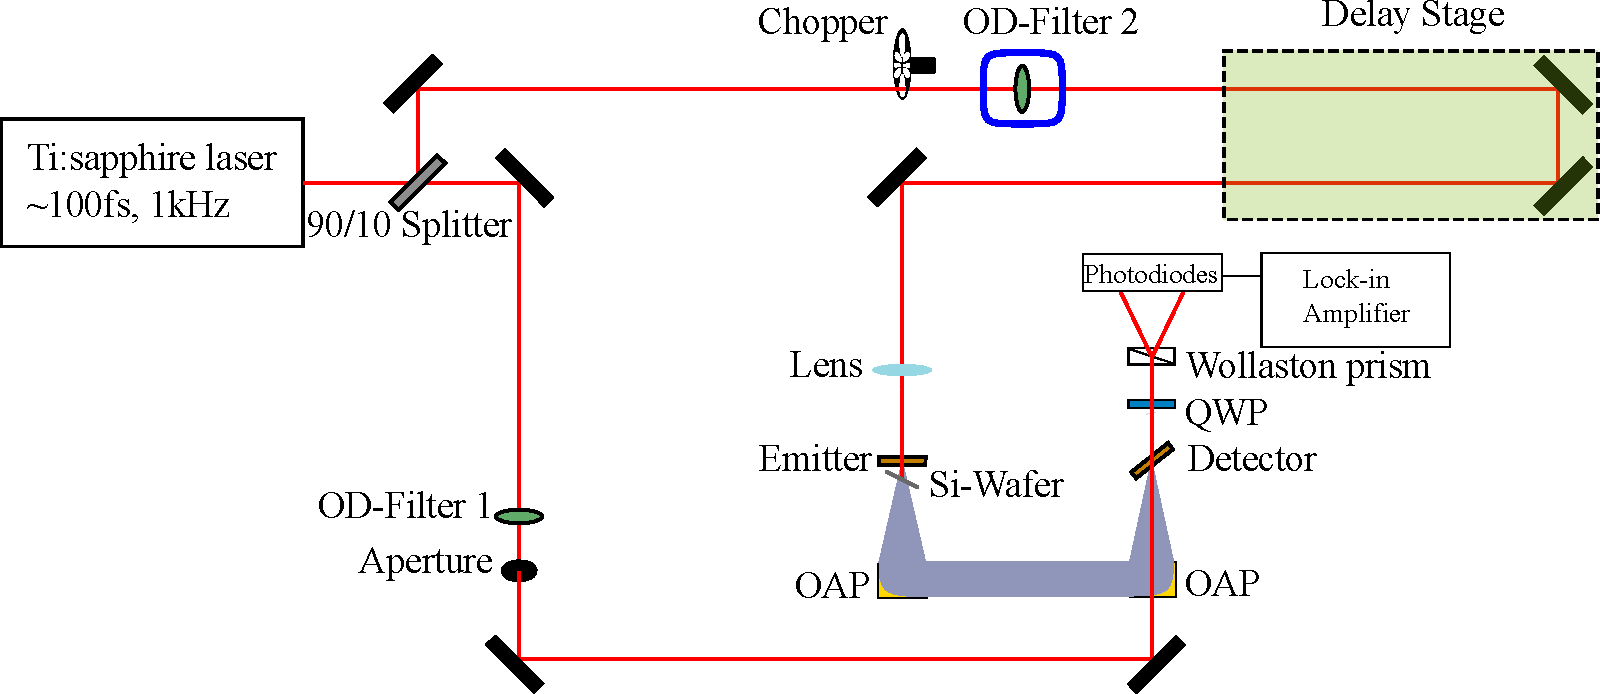
\includegraphics[width=\textwidth]{images/Aufbau_blue_square.pdf}
    \end{overprint}
  \end{figure}  
\end{frame}

\begin{frame}{Electric field}
  \begin{equation}
    \frac{\symup{\Delta}I}{I} = \text{sin}(\theta) = \frac{2\pi}{\lambda} n_0^3 l r E_\text{THz}
  \end{equation}
  \begin{columns}
    \begin{column}{.5\textwidth}
  \begin{figure}
    \begin{overprint}
      \onslide<1>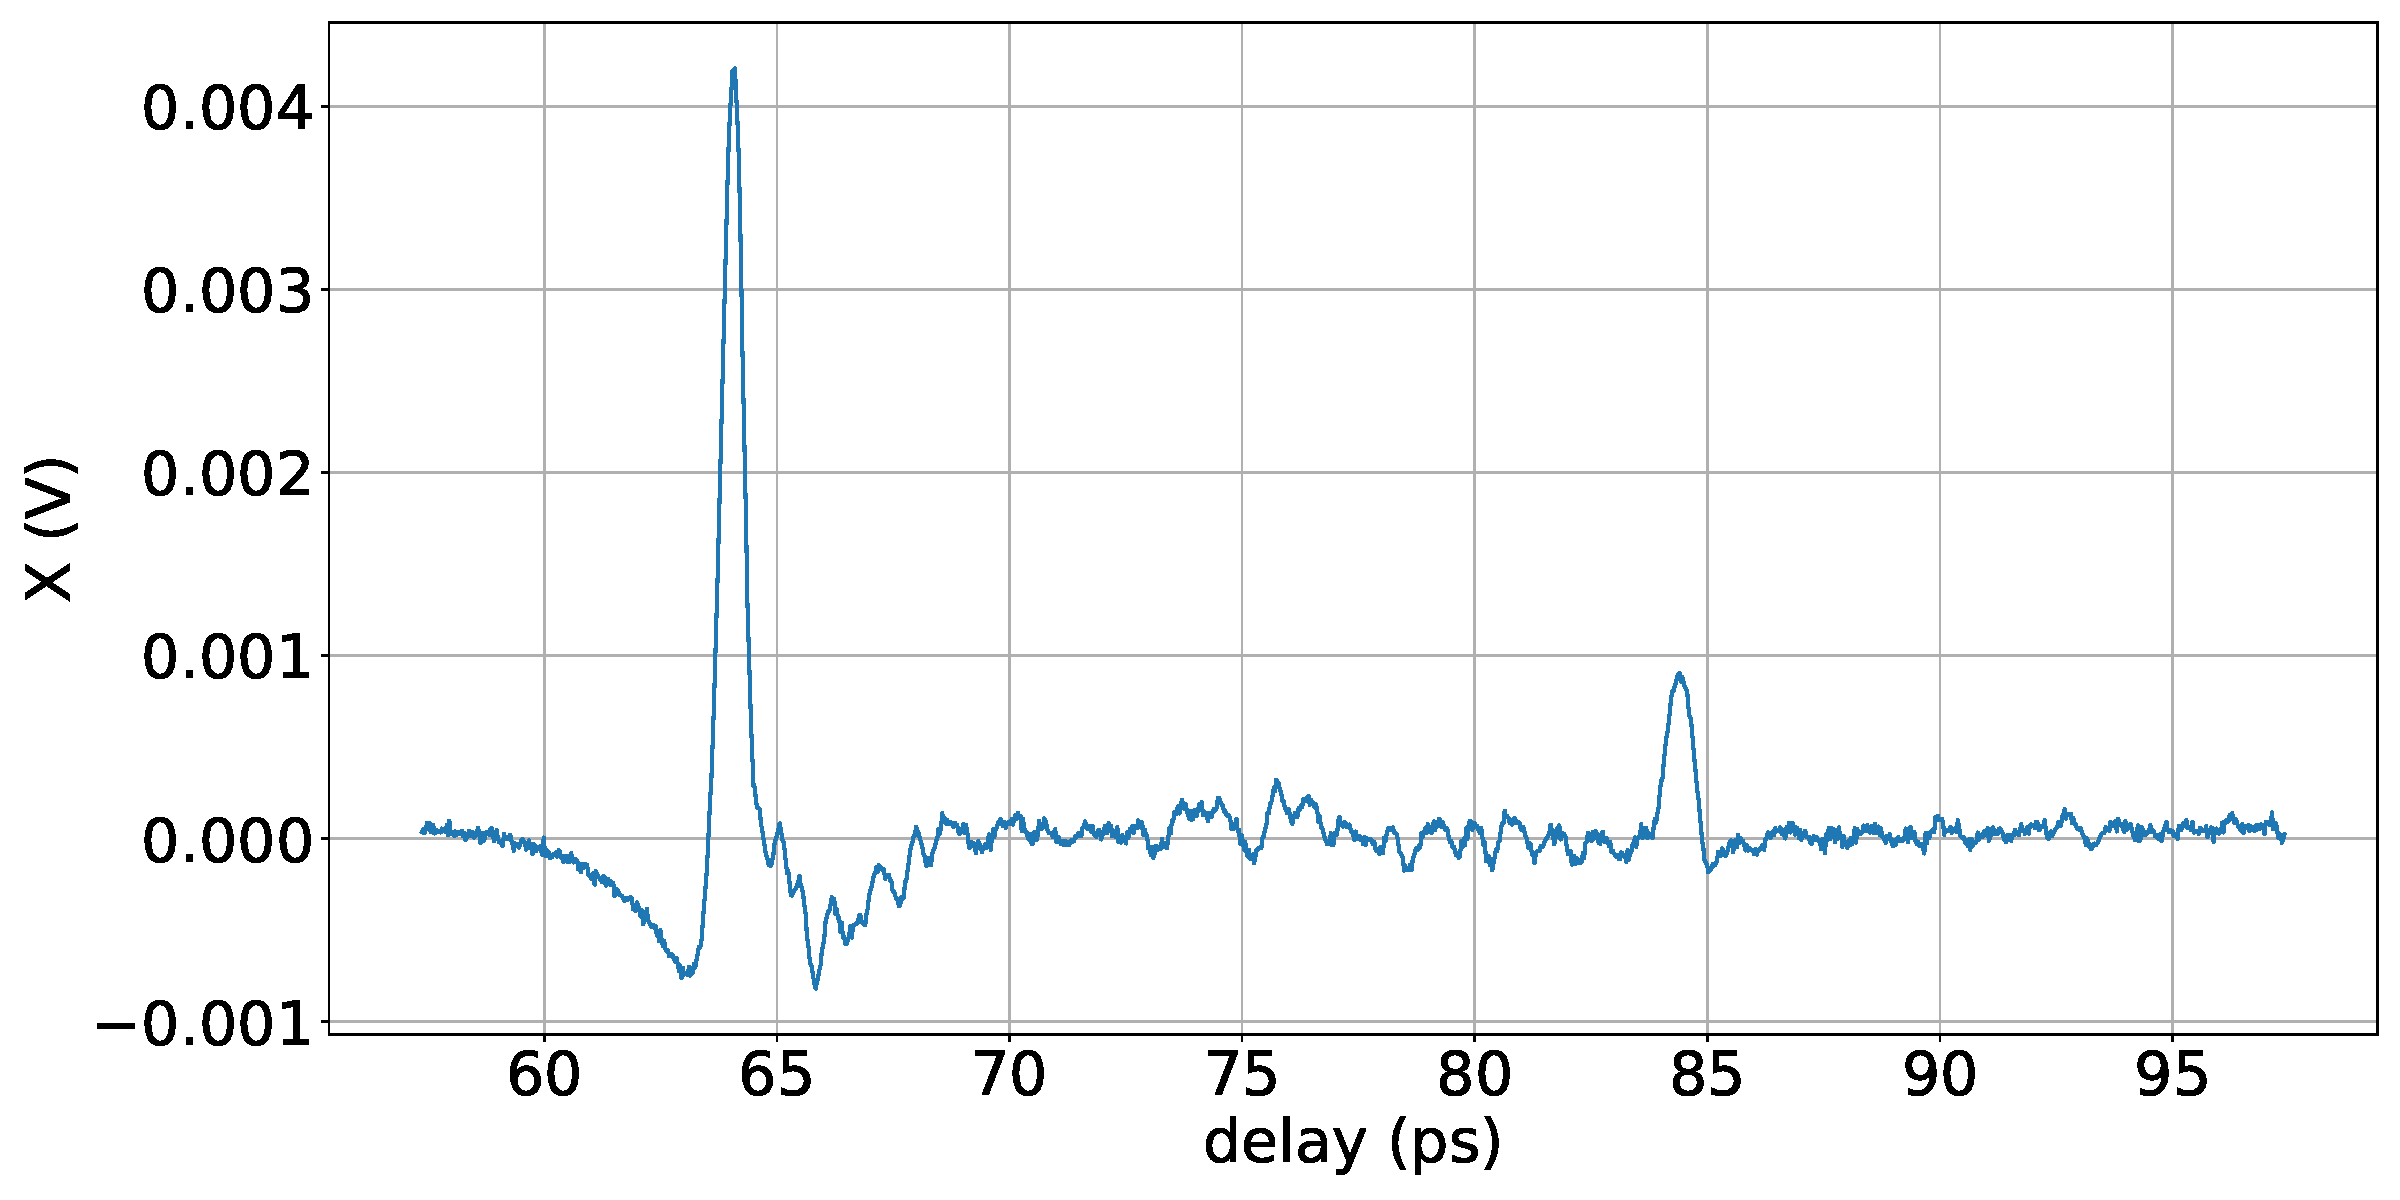
\includegraphics[width=\textwidth]{images/2_11_30_20normalX.pdf}
      \onslide<2>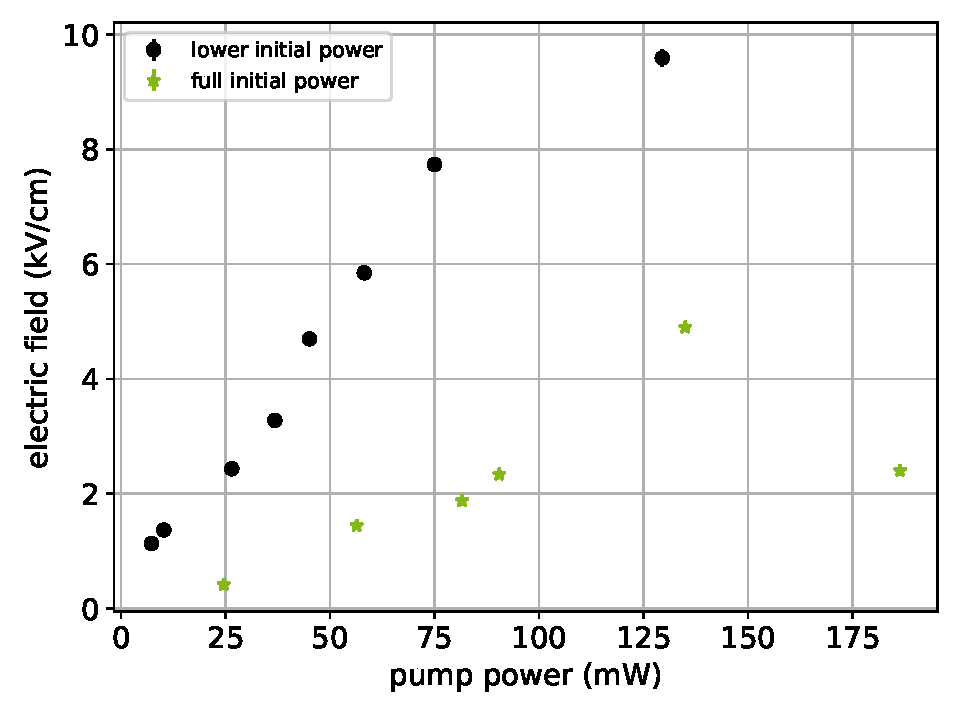
\includegraphics[width=\textwidth]{images/eltric_field_ZnTe.pdf}
    \end{overprint}
  \end{figure}
  \end{column}
  \begin{column}{.5\textwidth}
    \begin{figure}
      \begin{overprint}
        \onslide<1>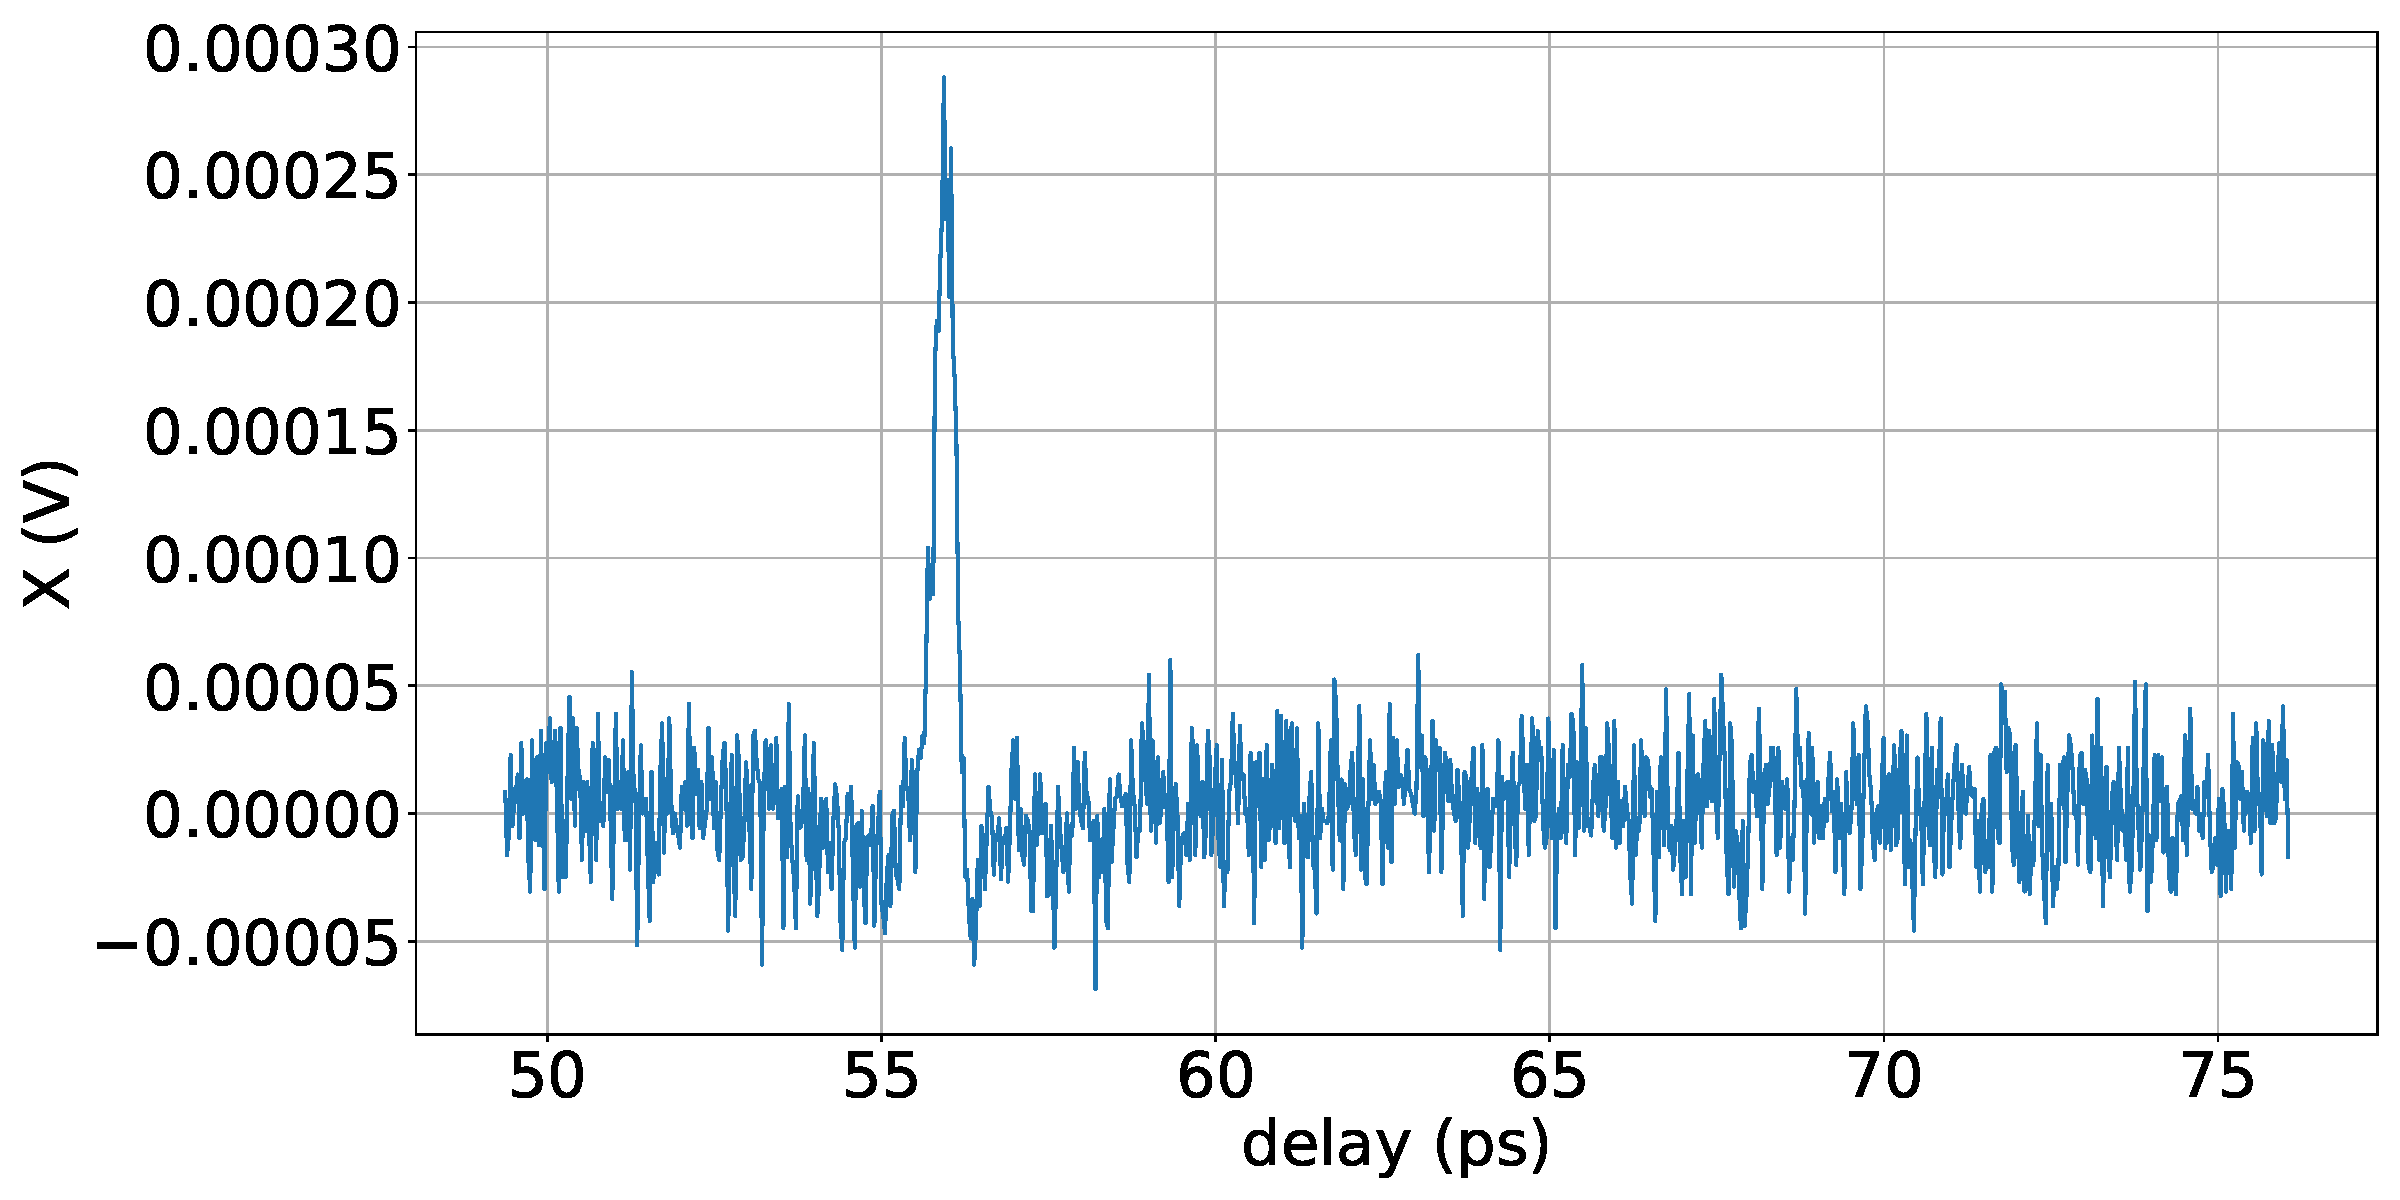
\includegraphics[width=\textwidth]{images/GaP14_55_42normalX.pdf}
        \onslide<2>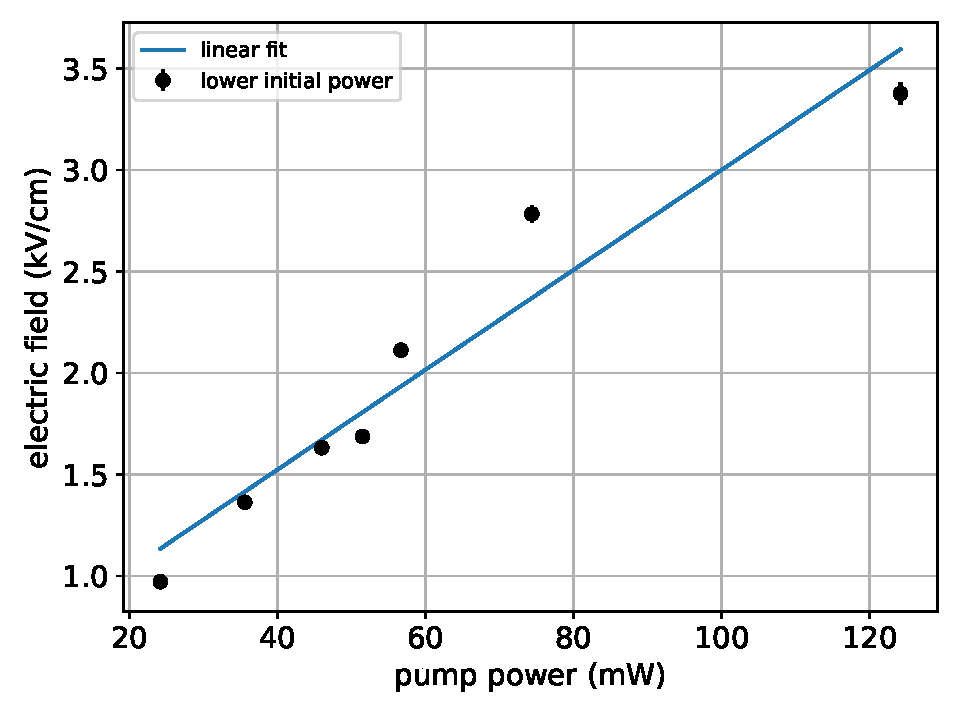
\includegraphics[width=\textwidth]{images/eltric_field_GaP.pdf}
      \end{overprint}
    \end{figure}    
  \end{column}
  \end{columns}
\end{frame}

\begin{frame}{Power}
  \begin{align}
    I_\text{THz} =& c \epsilon_0 E_\text{THz}^2 \\
    P =& \int\, I_\text{THz} \,\symup{d}A_\text{spot}\\
    P =& I_\text{THz}\cdot A_\text{spot}
\end{align}
  \begin{columns}
    \begin{column}{.5\textwidth}
  \begin{figure}
    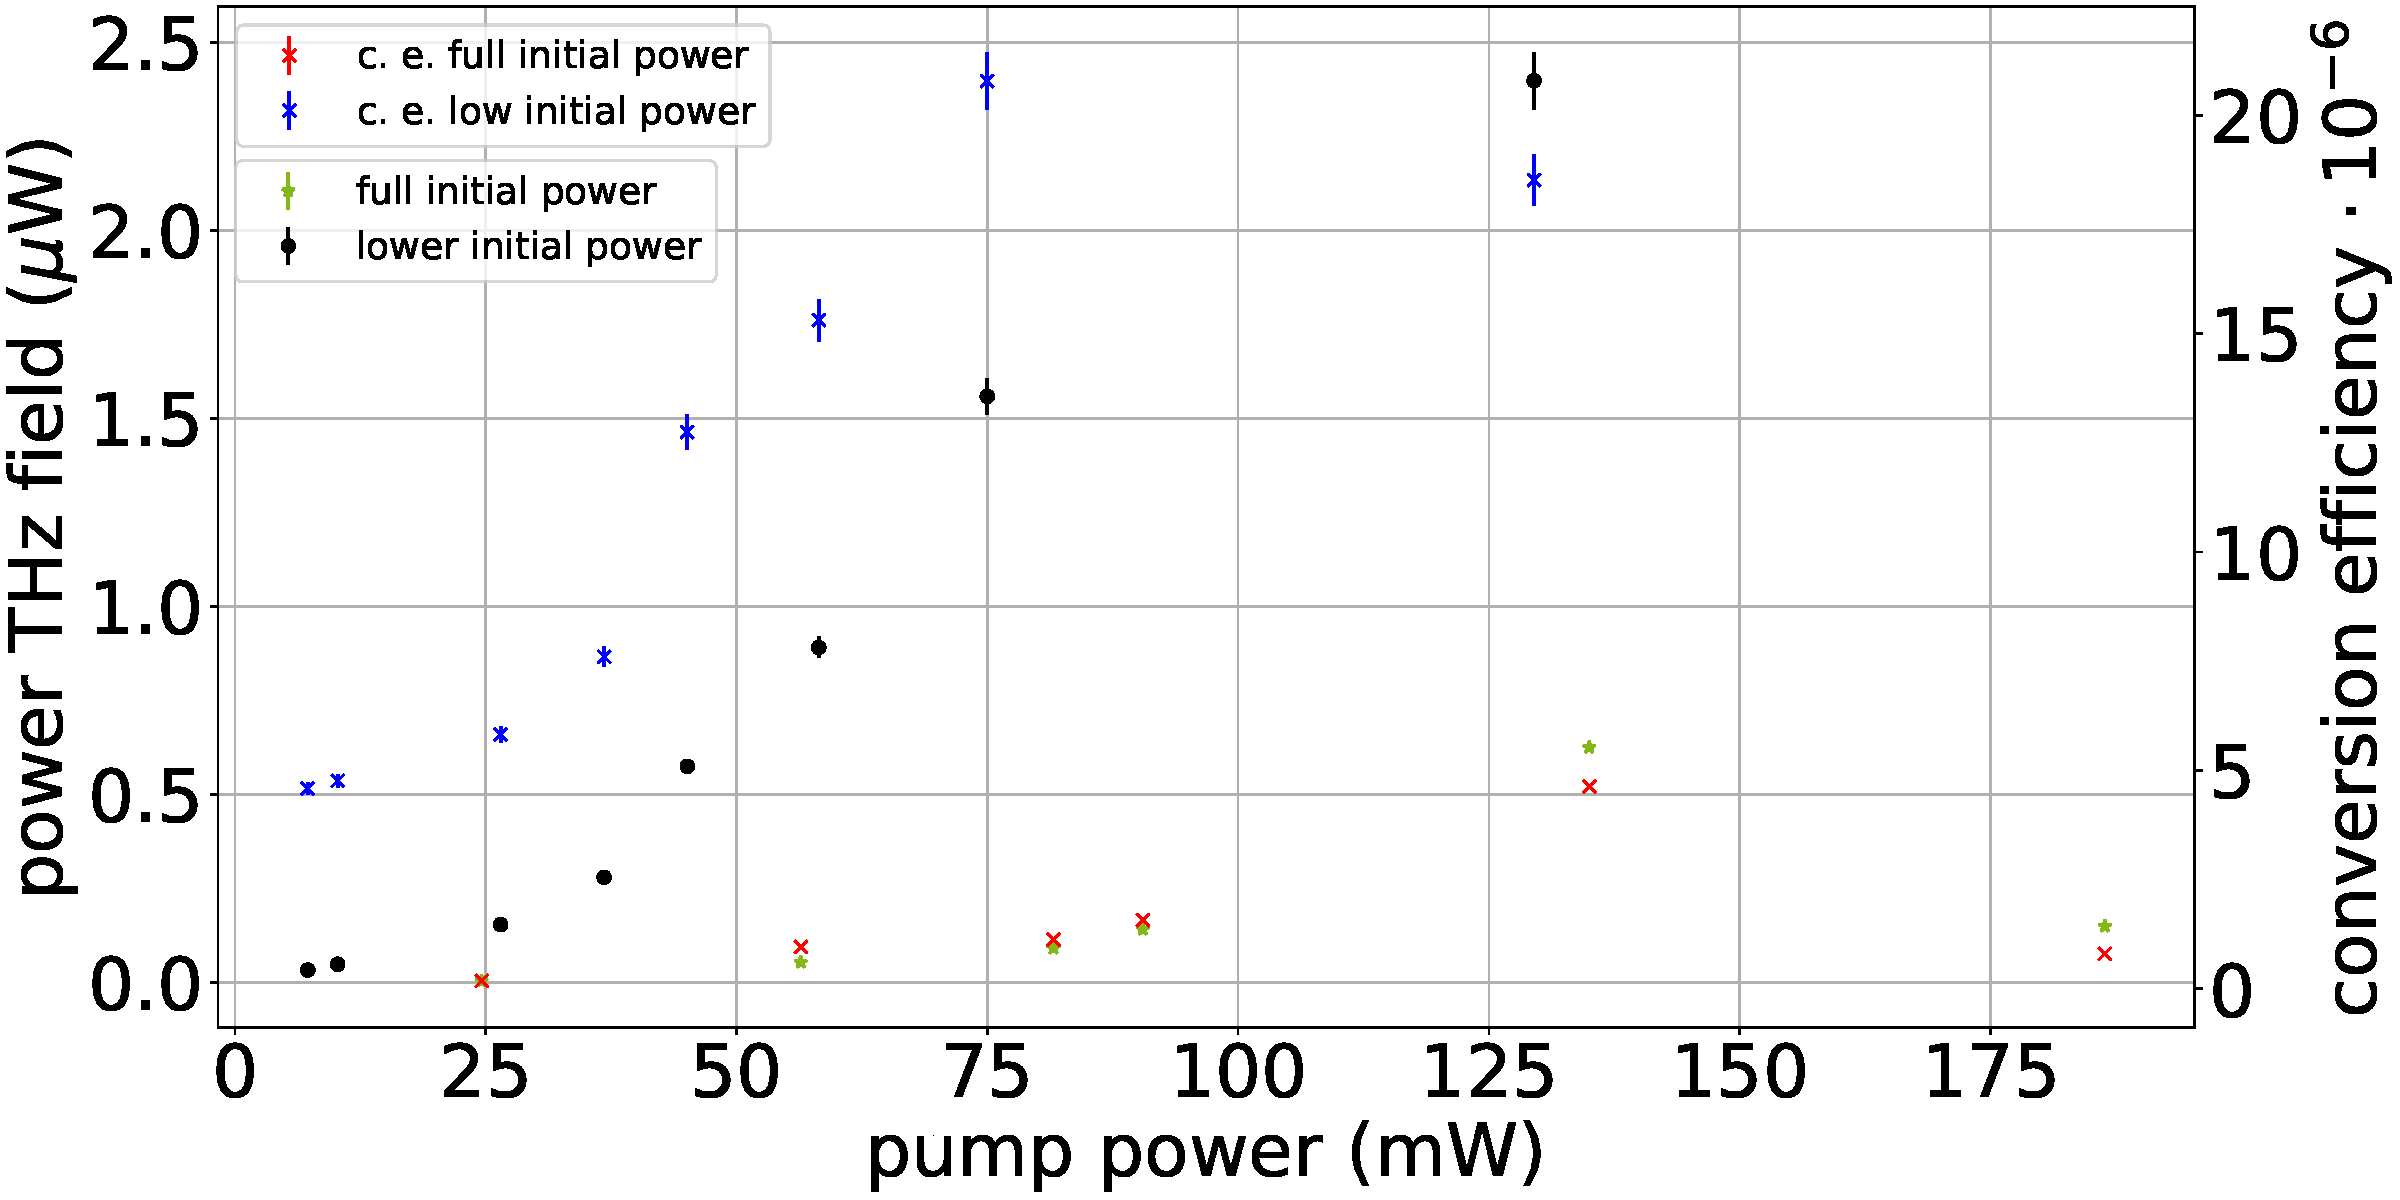
\includegraphics[width=\textwidth]{images/Powerznte.pdf}
  \end{figure}
  \end{column}
  \begin{column}{.5\textwidth}
    \begin{figure}
      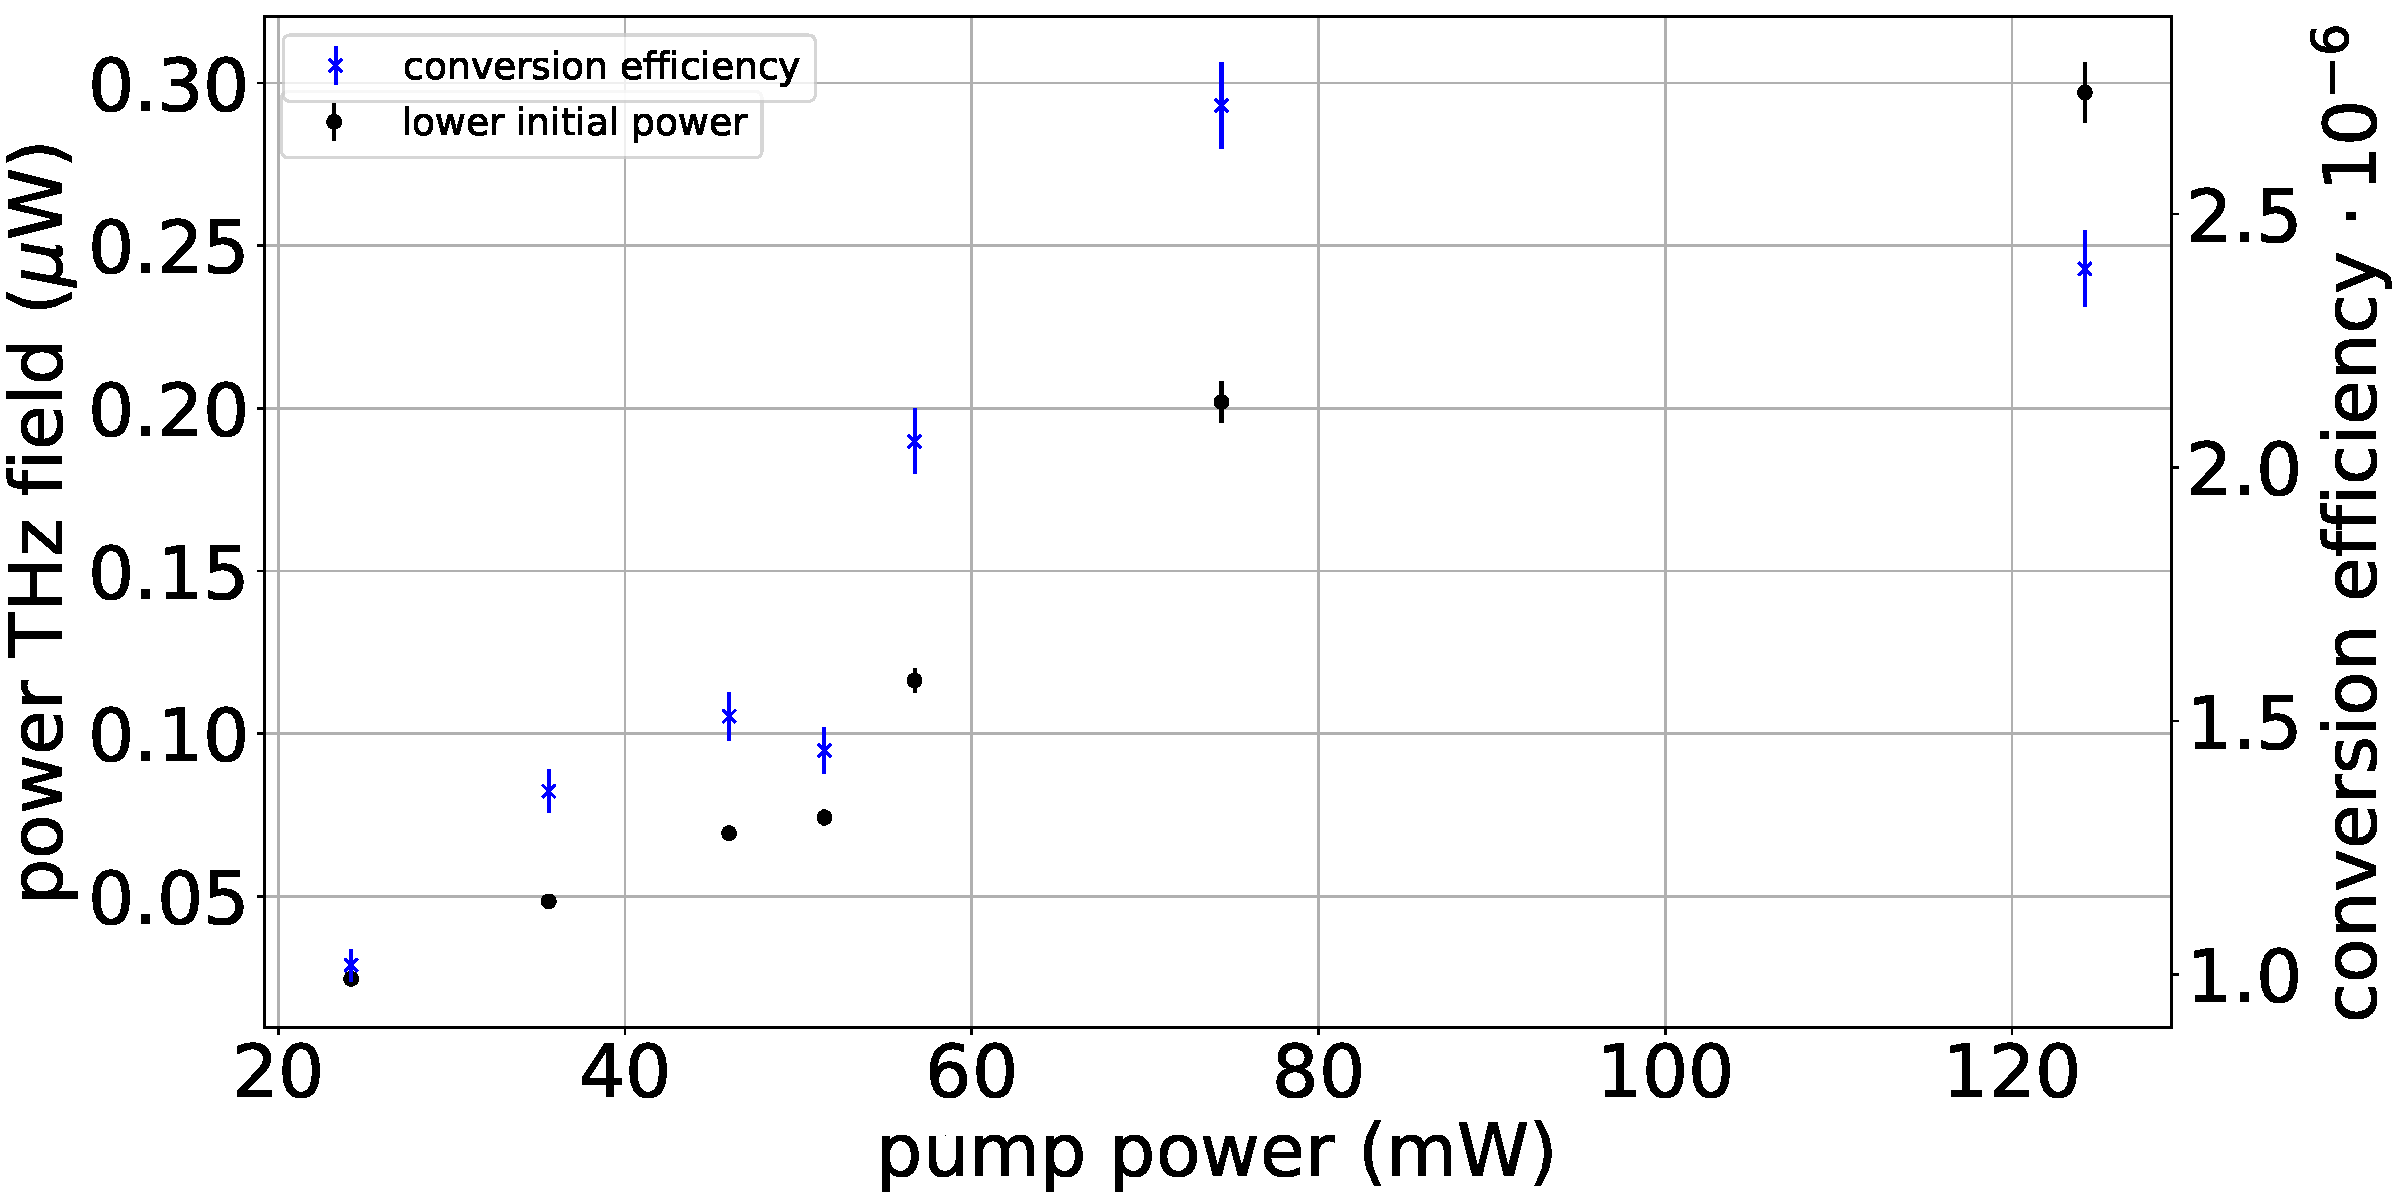
\includegraphics[width=\textwidth]{images/Powergap.pdf}
    \end{figure}    
  \end{column}
  \end{columns}
\end{frame}

\section{Sources}
\printbibliography
\end{document}
